% !TeX spellcheck = it_IT
\documentclass[a4paper,12pt,oneside]{book}
\usepackage{amsmath}
\usepackage{graphicx}
\usepackage{float}
\usepackage[hyphens]{url}
\usepackage[hidelinks]{hyperref}
\usepackage{siunitx}
\usepackage{setspace}
\usepackage{wrapfig}
\usepackage[english,italian]{babel}
\usepackage[utf8]{inputenc}
\usepackage{ fancyhdr }
\usepackage{pdfpages}
\usepackage{titlesec}
\usepackage{wrapfig}
\usepackage{tabularx}
\addto\captionsitalian{\renewcommand{\bibname}{Riferimenti bibliografici e sitografici}}
\onehalfspacing
%\doublespacing
\fancypagestyle{plain}{
%	\renewcommand{\headrulewidth}{0pt}
	\fancyhead[L]{}
	\fancyfoot[R]{\thepage}}
	\cfoot{}
	\chead{}
\pagestyle{plain}

\usepackage{geometry}
\geometry{
	a4paper,
	total={140mm,207mm},
	left=40mm,
	top=50mm,
	right=30mm,
	bottom=40mm
}

%\titleformat{\chapter}[display]
%{\normalfont\bfseries}{}{0pt}{\Huge}

\makeatletter 
\renewcommand{\frontmatter}{% 
	\cleardoublepage\@mainmatterfalse 
	\pagenumbering{smallRoman}} 
\DeclareRobustCommand{\@smrc}[1]{% 
	\begingroup$\m@th$\fontsize{\sf@size}{\sf@size}\selectfont#1\endgroup} 
\def\smallRoman#1{\expandafter\@smallRoman\csname c@#1\endcsname} 
\def\@smallRoman#1{\@smrc{\expandafter\@slowromansmallcap\romannumeral #1@}} 
\def\@slowromansmallcap#1{\ifx @#1% then terminate 
	\else 
	\if i#1I\else 
	\if v#1V\else 
	\if x#1X\else 
	\if l#1L\else 
	\if c#1C\else 
	\if d#1D\else 
	\if m#1M\else 
	#1\fi\fi\fi\fi\fi\fi\fi 
	\expandafter\@slowromansmallcap 
	\fi 
} 
\makeatother
\begin{document}

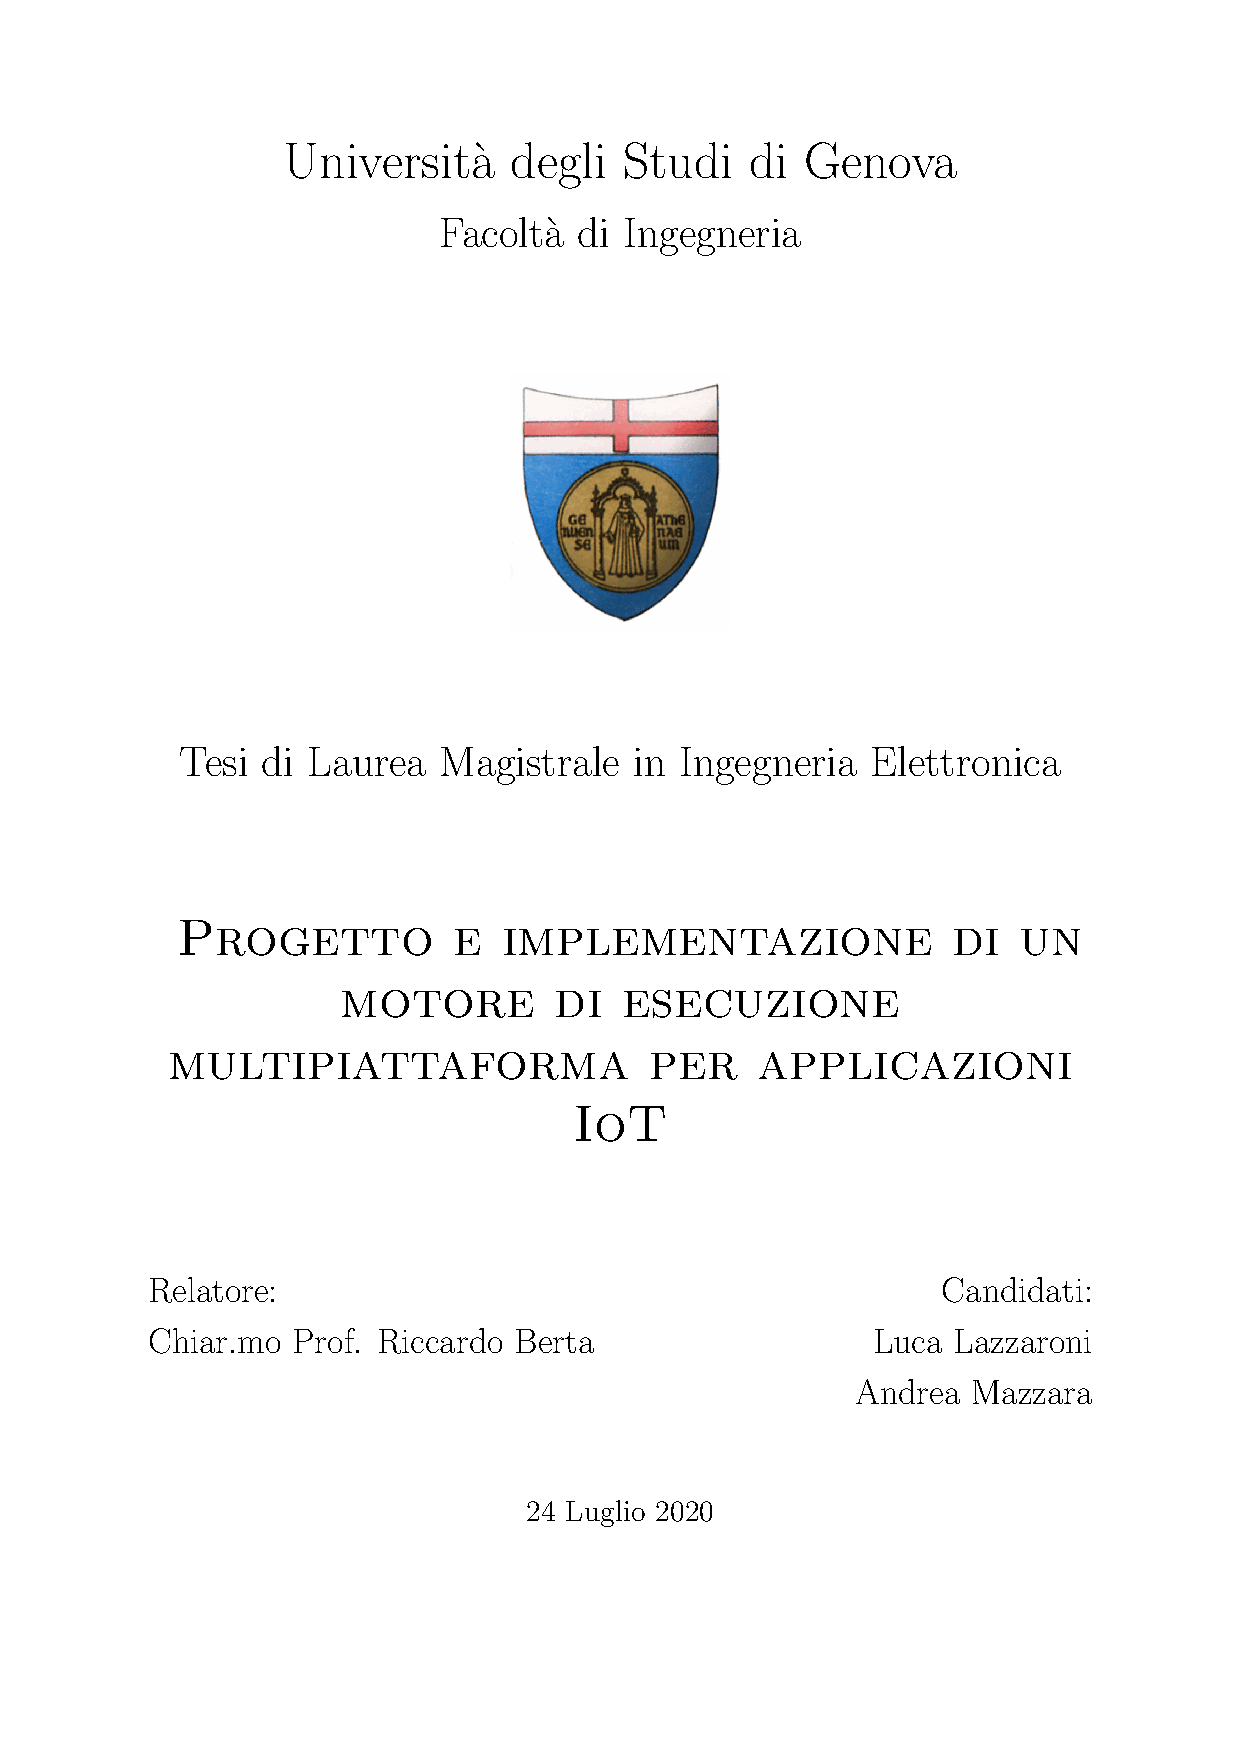
\includepdf{paginaIniziale}

\vfill

\newpage\null\thispagestyle{empty}\newpage

\frontmatter
\thispagestyle{empty}
\null\vspace{\stretch {1}}
\begin{center}
	\section*{\centering Ringraziamenti}
		Ringraziamenti.
\end{center}
\vspace{\stretch {2}}\null
\newpage
\thispagestyle{empty}
\begin{flushright}
	\null\vspace{\stretch {1}}
	Dedica 
	\vspace{\stretch {2}}\null
\end{flushright}

\clearpage
%\fancypagestyle{plain}{\fancyhead{}\renewcommand{\headrulewidth}{0pt}}
\renewcommand{\headrulewidth}{0pt}
%\null\vspace{\stretch {1}}
\begin{center}
	\huge{\textbf{Sommario}}
\end{center}
\null\vspace{\stretch {1}}

\begin{spacing}{1.25}
	
Le applicazioni dell'Internet of Things (IoT) richiedono spesso una notevole larghezza di banda, bassa latenza e performance affidabili, e al tempo stesso devono rispettare requisiti normativi e di conformità, motivo per cui il Cloud Computing non risulta adatto in questi particolari casi applicativi.

Per ovviare ai problemi sopracitati, negli ultimi anni si sta affermando un nuovo approccio, l'Edge Computing: un’architettura distribuita di micro data center, ciascuno in grado di immagazzinare ed elaborare i dati a livello locale e, in seguito, trasmetterli ad un data center centralizzato o a un database su Cloud.

Edge Engine nasce allo scopo di realizzare un motore il più generico possibile e slegato dall'hardware, tale da raccogliere dati provenienti dai dispositivi ad esso collegati, elaborarli e inviarli su Cloud.

In questo specifico caso si tratterà lo sviluppo di Edge Engine per dispositivi di tipo PC (Windows/ Linux/ MacOS). Il linguaggio di programmazione utilizzato sarà il C++, con l'intento di ottenere un prodotto finale multipiattaforma, caratteristica concorde con i requisiti preposti di genericità e indipendenza dall'hardware.

Una volta completato lo sviluppo del sistema, ne verranno testate le potenzialità prima in un contesto reale, per poi passare ad un ambito virtuale. Nel primo caso si utilizzerà l'engine per il trattamento di dati provenienti da PC (info su RAM e ROM). Nel secondo invece, verrà creato un componente su Unity3D in grado di usufruire dei servizi offerti da Edge Engine, ma applicati a dati ottenuti dalla scena di gioco.

In ultimo, al fine di ottenere un resoconto riguardo l'effettiva efficacia del sistema, oltre che possibili spunti su eventuali criticità, verrà illustrato un esempio di utilizzo della libreria, in ambiente Arduino, da parte di due tesisti triennali.
\end{spacing}
\null\vspace{\stretch {2}}
\clearpage
\renewcommand{\headrulewidth}{0.5pt}


\begingroup
\fancypagestyle{plain}{\fancyhead{}\renewcommand{\headrulewidth}{0pt}}
\tableofcontents
\listoffigures
\listoftables
\cleardoublepage
\endgroup
\mainmatter
\chapter{Introduzione}
Negli ultimi anni, la mole di dati prodotta da aziende e privati sta crescendo esponenzialmente, tanto che, entro il 2022, si stima che in media si avranno 50 dispositivi connessi a Internet per abitazione \ref{iotedge}. Ovviamente questi dati necessitano di essere processati e conservati, oltre che condivisi tra più dispositivi all'occorrenza. A tal fine, la modalità che si è adottata maggiormente negli ultimi anni è quella del Cloud Computing: i dati non vengono processati in locale per mancanza di risorse, ma inviati a specifici data center online in grado di elaborarli e processarli, oltre che conservarli. Tale approccio introduce però alcune criticità:
\begin{itemize}
	\item \textbf{Latenza}: in molti ambiti è richiesta un'elaborazione dei dati in tempo reale, si pensi per esempio ad un'eventuale applicazione che permetta a un veicolo autonomo di riconoscere i pedoni. In questo specifico caso è richiesta una bassissima latenza dato l'enorme rischio in gioco. Tuttavia, proprio l'invio dei dati al Cloud, la successiva elaborazione degli stessi e, infine, l'invio di un feedback al dispositivo in uso, introducono ritardi non trascurabili, pertanto in questi specifici casi il Cloud Computing risulta non essere l'approccio migliore.
	\item \textbf{Scalabilità}: l'invio dei dati al Cloud è problematico in tal senso, dato soprattutto il numero in crescita esponenziale di dispositivi connessi. Inoltre, l'invio di tutti i dati al Cloud è inefficiente in termini di consumo di risorse, in particolare se non tutti i dati sono necessari al Deep Learning.
	\item \textbf{Privacy}: l'invio di dati sensibili a server online aumenta i rischi di furto di tali informazioni, oltre al fatto che l'utente spesso e volentieri non è a conoscenza di come questi dati verranno trattati né tantomeno di dove saranno conservati.
\end{itemize}
Una possibile soluzione a queste tre criticità, proprie del Cloud Computing, è l'Edge Computing (vedi figura \ref{edge}). 
\begin{figure}[H]
	\centering
	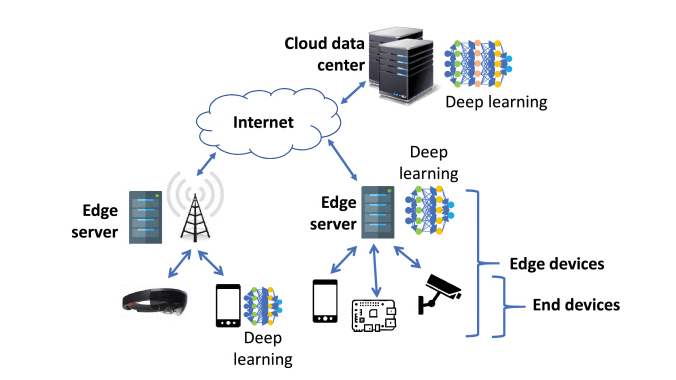
\includegraphics[width=\linewidth, height= 0.3 \textheight]{pics/edgecomputing.jpeg}
	\caption{Struttura dell'Edge Computing}
	\label{edge}
\end{figure}
Tale approccio prevede una rete di micro data center posti nelle vicinanze dei dispositivi che rilevano i dati da elaborare. Proprio questa vicinanza alle sorgenti dei dati permette di ridurre drasticamente la latenza (si veda figura \ref{edgevs}). Inoltre, al fine di incrementare le prestazioni in termini di scalabilità, è prevista una struttura gerarchica dei dispositivi connessi, oltre al fatto che non è necessario apportare modifiche o espansioni ai data center in Cloud siccome i dati vengono elaborati in locale. Per quanto riguarda infine i vincoli di privacy, l'Edge Computing prevede l'elaborazione dei dati alla sorgente, solitamente grazie a un server locale, perciò i dati non vengono trasmessi sulla rete globale, riducendo dunque i rischi che ne deriverebbero.
\begin{figure}[H]
	\centering
	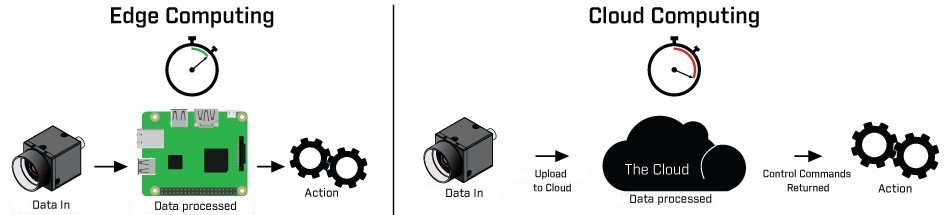
\includegraphics[width=\linewidth, height= 0.15 \textheight]{pics/edgevscloud.jpeg}
	\caption{Confronto tra Edge e Cloud Computing}
	\label{edgevs}
\end{figure}
L'approccio Edge Computing presenta però alcune criticità.\\
Uno degli aspetti più importanti da considerare è l'elevata quantità di risorse richiesta da determinati algoritmi (come ad esempio quelli di Machine Learning o di elaborazione delle immagini), in contrapposizione con l'utilizzo di nodi locali dotati di ridotta potenza di calcolo rispetto ai server centralizzati.\\
Un secondo problema è la coordinazione tra i dispositivi Edge e il Cloud, considerando che per ognuno di essi si avranno verosimilmente differenti capacità di calcolo e tipologie di connessione alla rete.\\
In ultimo, dal lato privacy, anche se le potenziali minacce sono ridotte rispetto a una soluzione unicamente basata sul Cloud Computing, la riservatezza rimane comunque un punto delicato poiché i dati necessitano di essere condivisi tra i vari dispositivi e pertanto risulta necessario l'utilizzo della comunicazione in rete, oltre al fatto che il dispositivo perimetrale avrà meno potenza di calcolo da dedicare a complessi algoritmi di criptazione.\\
Con queste premesse nasce l'idea di realizzare Edge Engine: un runtime system generico, slegato dall'hardware, in grado di interpretare codice per dispositivi multipiattaforma, comprese board di sviluppo per microcontrollori. Tale sistema è in grado di elaborare i flussi di dati provenienti dai sensori ad esso collegati grazie all'utilizzo degli script: insiemi di operazioni prestabilite che possono anche essere composte al fine di eseguire calcoli complessi sui dati in ingresso. L'Edge Engine è configurato in modo tale da recuperare dal Cloud gli scripts associati al dispositivo in uso, eseguirli localmente e poi trasmettere nuovamente al Cloud i risultati ottenuti. Per il corretto funzionamento di Edge Engine è dunque necessario un server online che conservi gli scripts e le descrizioni dei vari dispositivi. In questo specifico caso verrà utilizzato Measurify: una piattaforma cloud creata dall'Elios Lab dell'Università di Genova per gestire oggetti smart dell'Internet of Things (IoT).\\
Lo scopo del progetto in esame sarà la realizzazione di Edge Engine per sistemi PC (Windows/Linux/MacOS) e, successivamente, l'impiego di tale motore in un contesto di realtà virtuale, quale un simulatore medico, in modo da illustrare e testare un'ulteriore modalità di impiego del sistema.
\begin{figure}[H]
	\centering
	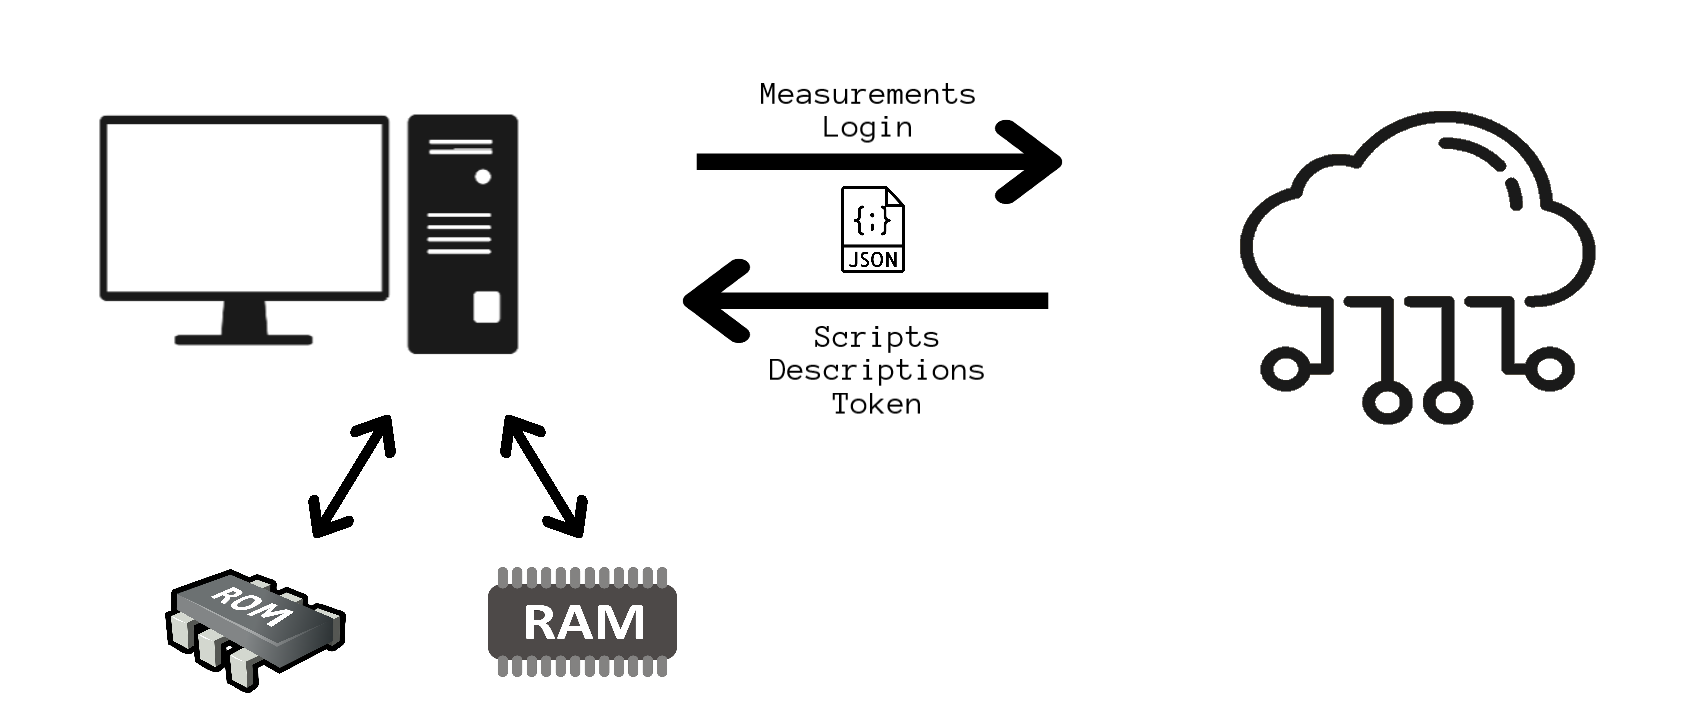
\includegraphics[width=\linewidth, height= 0.25 \textheight]{pics/edgine}
	\caption{Edge Engine per PC}
	\label{edgine}
\end{figure}
\fancypagestyle{plain}{\fancyhead{}\renewcommand{\headrulewidth}{0pt}}
\chapter{Stato dell'Arte}
In un mondo in cui sempre più dispositivi necessitano di connessione alla rete e i dati personali richiedono un alto livello di protezione, oltre che di elaborazione attraverso l'impiego di algoritmi più o meno complessi, le potenzialità offerte in tale direzione dall'Edge Computing hanno attirato l'attenzione dei colossi del settore.

Google, ad esempio, ha recentemente rilasciato Edge TPU e Cloud IoT Edge \cite{iotgoogle}: il primo è un ASIC creato specificamente per eseguire l'IA a livello periferico, mentre il secondo è una piattaforma per l'Edge Computing che estende le capacità di elaborazione dei dati e Machine Learning (ML) di Google Cloud ai dispositivi perimetrali. L'idea di fondo è quella di costruire i propri modelli sul Cloud, per poi utilizzarli su dispositivi Cloud IoT Edge sfruttando le potenzialità offerte dall'acceleratore hardware Edge TPU. Tale circuito è inoltre in grado di eseguire TensorFlow Lite \cite{tflowlite}: una piattaforma che fornisce un set di strumenti i quali permettono all'utente di convertire modelli di reti neurali TensorFlow in versioni semplificate e ridotte, adatte ai dispositivi Edge \cite{tflowres}.

Amazon, all'interno della sua offerta di servizi Cloud (AWS), mette a disposizione la soluzione IoT Greengrass \cite{aws}, che semplifica l'inferenza di ML in locale sui dispositivi, mediante modelli creati, formati e ottimizzati nel Cloud. L'utente può inoltre utilizzare modelli il cui training viene fatto in prima persona. L'AWS IoT Greengrass dispone del runtime Lambda \cite{lambda}: un gestore di messaggi, accesso alle risorse, ecc. I requisiti minimi a livello hardware sono 1 GHz di frequenza del processore e 128 MB di RAM.

Microsoft mette a disposizione Azure IoT Edge \cite{azure}: un servizio che permette di distribuire i carichi di lavoro del Cloud per eseguirli su dispositivi perimentrali dell'IoT. Il codice di IoT Edge supporta numerosi linguaggi tra cui C, C\#, Java, Node.js e Python, inoltre la latenza è ridotta siccome i dati vengono elaborati in locale, con la possibilità di usare l'architettura hardware Microsoft, Project Brainwave \cite{bwave}. I dispositivi perimetrali possono poi anche funzionare in condizioni di connessione a internet scarsa, grazie alla gestione dei dispositivi di Azure che sincronizza in automatico lo stato più recente degli apparecchi dopo la riconnessione a internet. Microsoft ha inoltre rilasciato EdgeML \cite{edgeml}: una suite di algoritmi di ML progettata per un utilizzo in situazioni di risorse ridotte. I risultati pubblicati sull'uso di EdgeML per il training su Cloud in condizioni di limitata potenza di calcolo \cite{edgemlres}. Al momento tale libreria prevede algoritmi di tipo k-Nearest Neighbors (kNN) per classificazione, regressione e ranking noti con i nomi di Bonsai, ProtoNN e Robust PCA \cite{edgemlalg}.

In ultimo, IBM ha sviluppato IBM Edge Application Manager \cite{IBM}: una piattaforma intelligente, sicura e flessibile che fornisce uno strumento di gestione per l'elaborazione perimetrale. La soluzione proposta è autonoma, ossia consente ad un singolo amministratore di gestire scalabilità, variabilità e frequenza di modifica degli ambienti delle applicazioni su decine di migliaia di endpoint. Gli endpoint perimetrali si eseguono su contenitori Red Hat OpenShift \cite{redhat}. IBM Edge Application Manager supporta inoltre tool di IA per Deep Learning e riconoscimento di voce e immagini, oltre all'analisi video e acustica.

Anche nella letteratura scientifica è possibile reperire numerosi articoli pubblicati nel periodo recente, a indicare un orientamento in direzione Edge Computing.

In particolare, riguardo la possibilità di eseguire codice multipiattaforma che sfrutti le potenzialità offerte da questo approccio, si fa riferimento ad un articolo riguardante lo sviluppo di algoritmi di allocazione risorse per migliorare le prestazioni delle Vehicular Networks \cite{VN}. Per la selezione della piattaforma di esecuzione (es. Cloud Computing, Mobile Edge Computing, o Local Computing) viene utilizzato l'algoritmo k-Nearest Neighbor (kNN), mentre, per il problema di allocazione delle risorse computazionali, il Reinforcement Learning (RL). I risultati della simulazione mostrano che, rispetto all'algoritmo di base in cui tutte le attività vengono eseguite sul server di Edge Computing locale o mobile, lo schema di allocazione delle risorse consente una riduzione significativa della latenza che si attesta intorno all'80\%.

Per far fronte al problema del consumo di energia dei device IoT, l'approccio Edge Computing è stato trattato al'interno di un articolo di Olli Väänänen e Timo Hämäläinen \cite{energyIoT}. Aspetto importante di tale ricerca è la focalizzazione sul concetto di virtualizzazione. L'approccio consigliato è quello della container-based virtualization: ambienti di sviluppo virtuali emulano un determinato sistema operativo (OS), in questo modo è possibile produrre codice indipendente dalla piattaforma. I container possono essere eseguiti da dispositivi dotati di risorse limitate (es. Raspberry Pi), tuttavia richiedono una certa potenza computazionale e un generico OS.

Un ulteriore aspetto critico riguardante l'Edge Computing è il coordinamento tra dispositivi. Nell'ambito dei vari modelli che è possibile adottare, quelli tuple-based sono i più conosciuti e utilizzati, principalmente per la loro flessibilità \cite{tuple}. Ne è un esempio il modello Tusow (Tuple Spaces over the Web) \cite{tusow}. Le tuple rappresentano i messaggi o i dati scambiati tra i componenti e l'interazione tra gli stessi è gestita definendo come e quando i vari agenti coinvolti sono in grado di inserire, leggere o elaborare i dati. Tusow permette ai vari clients di rappresentare le tuple in diversi formati: YAML, JSON, XML, FOL e plain text. Il supporto multipiattaforma offerto da tale sistema mira a fornire un mezzo di interazione ad alto livello per clients eterogenei, permettendo agli sviluppatori di non curarsi delle complessità intrinseche della rete di basso livello.

La ricerca scientifica si sta orientando verso l'implementazione di algoritmi di ML applicati all'Edge Computing, come anche dimostrato dalle proposte di Google e Microsoft in tale ambito \cite{tflowres}, \cite{edgemlres}.
È stata ad esempio testata la possibilità di eseguire algoritmi di ML su Raspberry Pi \cite{mlrasp}. In particolare sono stati implementati tre algoritmi: Support Vector Machine (SVM), Multi-Layer Perceptron e Random Forest, raggiungendo una precisione oltre l'80\% mantenendo però un basso consumo di energia.

È stato inoltre analizzato un approccio di Deep Learning in cui vengono utilizzati autoencoder a livello Edge in modo da operare una riduzione delle dimensioni dei dati \cite{encoder}, portando benefici in termini di tempo e spazio richiesti. Tale progetto illustra tre differenti scenari. Nel primo, dati provenienti da sensori vengono mandati a dei "nodi Edge", dove viene applicata la riduzione delle dimensioni, per poi applicare le tecniche di ML su Cloud. Nel secondo, i dati che sono stati ridotti in Edge vengono trattati sul Cloud in modo da riottenere i dati originari per poi successivamente applicare il ML. Nel terzo ed ultimo caso invece, la tecnica utilizzata è quella del Cloud Computing: i dati vengono mandati dai sensori direttamente al Cloud. I risultati finali mostrano come l'utilizzo di autoencoder a livello Edge riduca il numero di features e, di conseguenza, l'ammontare di dati inviati al Cloud.

In ultimo, Respiro è un inalatore smart prodotto da Amiko \cite{respiro} che contiene un processore ultra-low-power ARM Cortex-M. Tale inalatore fa affidamento sul ML per interpretare le vibrazioni provenienti dal sensore posto al suo interno. Il dispositivo è addestrato per riconoscere diverse tipologie di respiro e calcolare di conseguenza importanti parametri in ambito medico come la capacità polmonare e la tecnica di inalazione. I dati così prodotti vengono poi processati da un'applicazione e, se la connessione lo permette, inviati al Cloud per essere conservati e elaborati potendoli confrontare inoltre con i risultati altrui a fini statistici. Infine, attraverso l'app, viene inviato un feedback all'utente affinché possa avere sotto controllo i dati estrapolati.

Queste sono le principali soluzioni disponibili nel mercato tecnologico e nelle più recenti ricerche accademiche. È possibile notare come gli aspetti ritenuti più importanti siano l'ottimizzazione delle risorse, il basso consumo di energia, l'indipendenza dalla piattaforma, la privacy e la bassa latenza, oltre alla facilità di utilizzo.

Edge Engine nasce con l'idea di base di creare un runtime system slegato dalla piattaforma che soddisfi i requisiti cardine dell'Edge Computing sopracitati. A differenza delle soluzioni appena presentate, questo progetto cerca di fornire un software completamente personalizzabile e adattabile a qualsiasi apparato IoT, come riassunto dallo schema visibile in figura \ref{edgecomplete}.

\begin{figure}
	\centering
	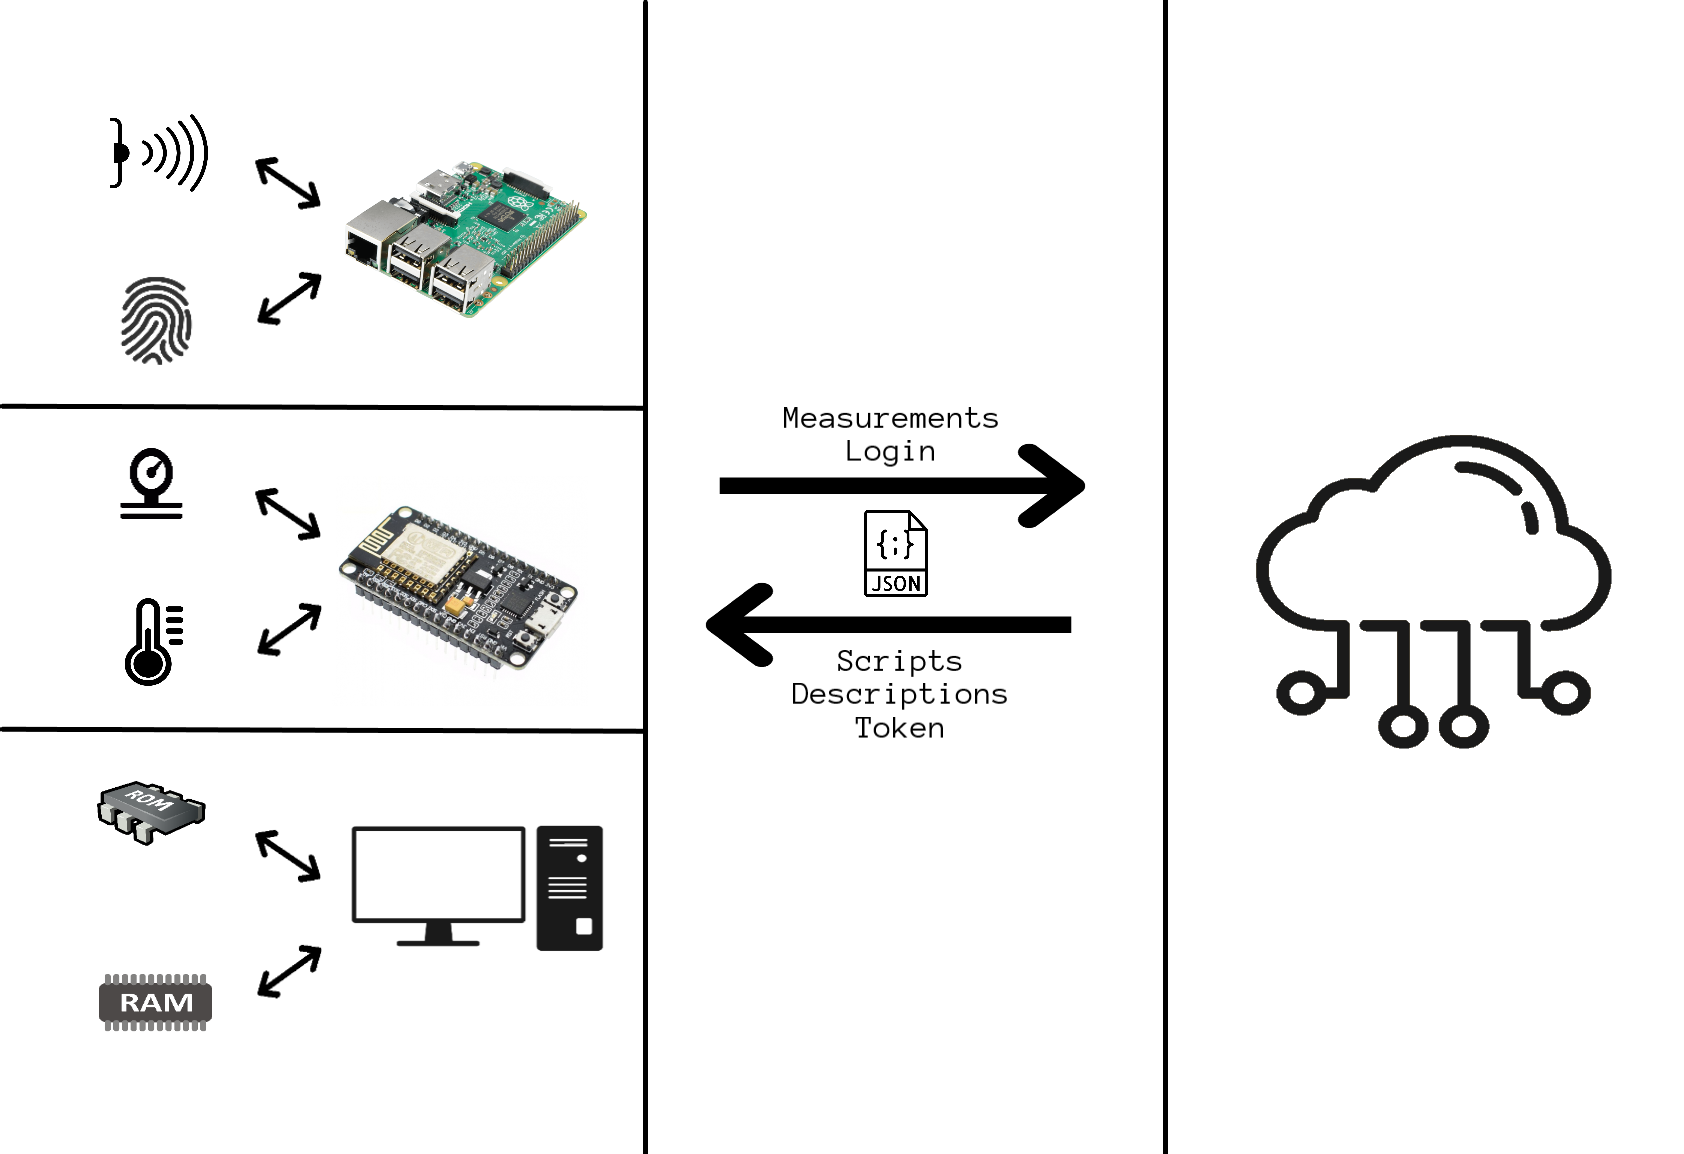
\includegraphics[width=\linewidth]{pics/edgineCP}
	\caption{Schema funzionale di Edge Engine su piattaforme eterogenee}
	\label{edgecomplete}
\end{figure}
\fancypagestyle{plain}{\fancyhead{}\renewcommand{\headrulewidth}{0pt}}
\chapter{Contesto di sviluppo}
In un contesto di Edge Computing, un ecosistema IoT necessita di tre componenti principali: un dispositivo che raccolga i dati dall'ambiente circostante tramite sensori, un motore di esecuzione in grado di interpretare tali informazioni e un server Cloud (si veda fig. \ref{ecosistema}). All'interno di quest'ultimo sono presenti le descrizioni dei device di interesse e, inoltre, vengono salvati i dati processati dall'engine.

\begin{figure}[H]
	\centering
	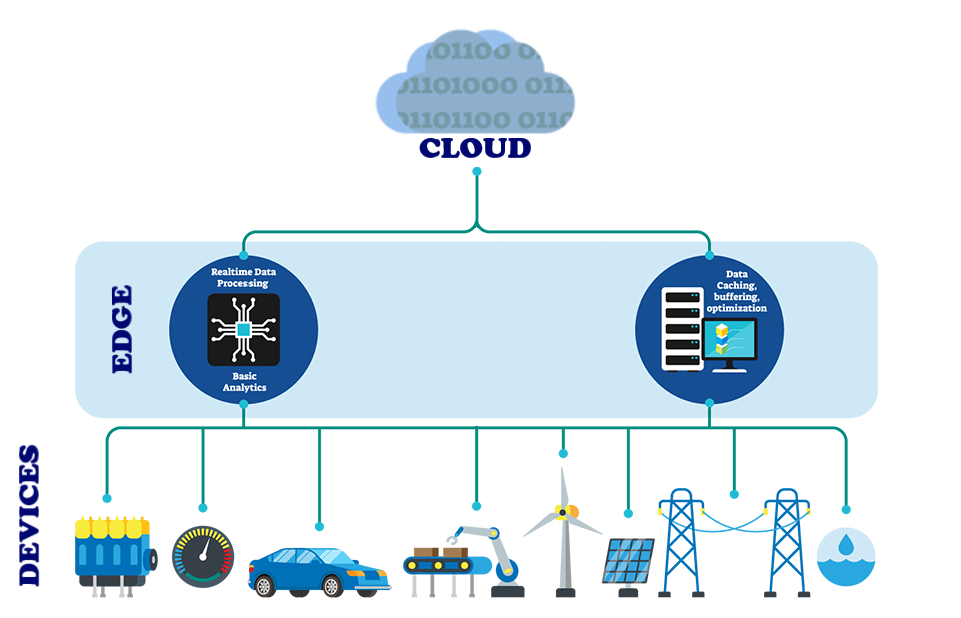
\includegraphics[width=0.8\linewidth]{pics/edgestructure}
	\caption{Ecosistema IoT basato sull'Edge Computing}
	\label{ecosistema}
\end{figure}

\section{Measurify}
Measurify è il server Cloud che è stato impiegato per questo progetto: una piattaforma Cloud-based, astratta e measurement-oriented creata dall'Elios Lab dell'Università degli Studi di Genova per gestire oggetti intelligenti negli ecosistemi IoT. Measurify modella tali oggetti come risorse web esponendole attraverso API che rispettano un'architettura REST (REpresentational State Transfer). In questo modo l'accesso remoto a dati e risorse avviene attraverso un'interfaccia HTTP(S), indipendente dalla piattaforma, per supportare lo sviluppo di applicazioni che si servono di tali oggetti. Le risorse delle API associate al dispositivo specifico sul quale il motore è in esecuzione sono configurabili da remoto con un'applicazione client (ad esempio una web application) che le modifica per gestire l'engine.

Per poter accedere a Measurify sono necessari un username ed una password che permettono di ricevere un token di sicurezza. Nel caso in questione si tratta di un JSON Web Token (JWT), che andrà inserito nell'header di tutte le richieste HTTP(S) successive per garantirne l'autorizzazione.

All'interno di Measurify è presente una struttura descrittiva dei dispositivi associati al proprio username  (si veda fig. \ref{cloudAPI}). Questa è composta da diversi campi che definiscono l'oggetto in questione:

\begin{itemize}
	\item \textbf{Thing}: è  l'oggetto generico che è soggetto a misurazioni da parte dei dispositivi (ad esempio una persona, una macchina, una casa, una città, ecc.);
	\item \textbf{Feature}: è la grandezza fisica misurata da un dispositivo (ad esempio il battito cardiaco, la temperatura ambientale, ecc.);
	\item \textbf{Device}: è un'istanza di una Board usata da una o più applicazioni che
	ha una descrizione virtuale sul Cloud API ;
	\item \textbf{Script}: è un file che contiene informazioni su come l'Edge Engine debba manipolare, memorizzare e trasmettere al cloud gli streams di dati provenienti dai sensori o da altri dispositivi. Può essere una funzione molto complessa per gli engine più potenti oppure un semplice insieme di parametri (ad esempio la velocità di acquisizione o il numero di dati da inviare assieme) per quelli di fascia inferiore;
	\item \textbf{Measurement}: è il valore di una grandezza fisica misurato dal sensore
	di un dispositivo per uno specifico oggetto;
\end{itemize}

\begin{figure}[H]
	\centering
	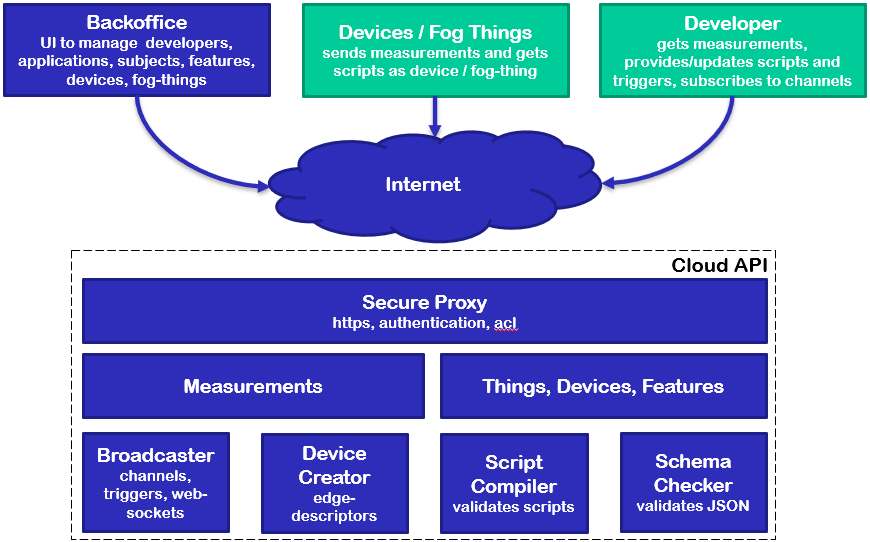
\includegraphics[width=\linewidth]{pics/cloudAPI}
	\caption{Architettura del server Cloud Measurify}
	\label{cloudAPI}
\end{figure}

\section{Edge Engine}
L'Edge Engine è composto da una serie di funzioni unite in un motore di esecuzione che viene eseguito su un host perimetrale. Il progetto è nato inizialmente con lo scopo di essere eseguito su piattaforme di fascia bassa. Di conseguenza, la prima versione ne prevedeva l’utilizzo solo su scheda di sviluppo ESP32-DevKitC V4 con modulo ESP32-WROVER-B su piattaforma Arduino, mantenendo però la possibilità di un futuro adattamento del codice a più dispositivi, come sarà mostrato nel capitolo successivo.

Il funzionamento dell'engine si può riassumere in macro-processi: accesso al Cloud, richiesta della propria descrizione virtuale, richiesta degli scripts da eseguire, lettura dati dai sensori, elaborazione locale dei dati, memorizzazione dei dati e invio degli stessi al Cloud.

L’engine, oltre a username e password necessari per l’accesso al Cloud, deve essere dotato di un identificativo univoco chiamato \textit{id}, inserito all'interno del codice, che gli permetta di identificare ed accedere alla propria rappresentazione virtuale e di specificare la provenienza di tutte le informazioni che andrà a comunicare.

In seguito all'autenticazione, l'engine deve richiedere la propria rappresentazione virtuale, che ne descrive l'identità, i parametri di configurazione e le funzionalità fornendo dunque gli identificativi degli scripts da eseguire. Sul Cloud, per ognuno di questi, deve essere stata in precedenza creata una risorsa di tipo \textit{script} che potrà essere ottenuta dall’engine tramite una GET request. Gli scripts e la descrizione virtuale sono tutti e soli gli elementi di configurazione aggiornabili da remoto. Una volta ottenuti può iniziare la fase operativa.

L’elaborazione locale dei dati raccolti avviene quindi attraverso gli scripts, una composizione di un set predefinito di operazioni semplici, la cui implementazione viene precaricata nell'engine. Queste possono essere applicate agli streams di dati nell'ordine desiderato per formare anche scripts complessi che producono in uscita nuovi streams. L'upload di questi dati sul Cloud può avvenire in due possibili modi: in modo continuo, ovvero il dato viene inviato non appena viene letto e/o processato oppure a lotti, ovvero si può specificare il numero di misure da raggiungere perché queste vengano inviate in blocco dopo essere state memorizzate una ad una.

L'invio dei dati avviene attraverso una POST request sulla rotta delle API dedicata, fornendo nel body della chiamata oltre al dato anche alcune informazioni di tracciabilità, come l'identificativo del dispositivo e dello script che lo ha generato.

Durante l’esecuzione potrebbero verificarsi dei malfunzionamenti che, in questi casi, dovranno essere comunicati dettagliatamente al Cloud, in modo da rendere noto se e quando questi si siano verificati. Così facenso si da anche la possibilità di prendere le dovute contromisure per correggere alcuni errori o semplicemente interpretare correttamente alcune situazioni inaspettate come l'assenza prolungata di comunicazioni verso il server da parte del dispositivo, che potrebbe essere dovuta a molteplici problematiche (connessione, autenticazione fallita, server temporaneamente offline, ecc.).

In figura \ref{edgecloud} è possibile vedere una struttura schematica dell'architettura del sistema Edge Engine - Measurify.

\begin{figure}[H]
	\centering
	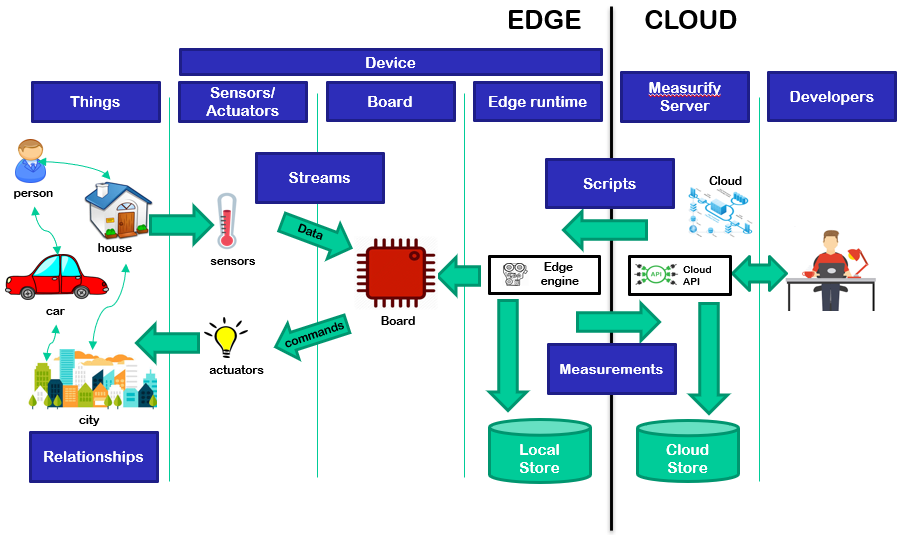
\includegraphics[width=\linewidth]{pics/edgearch}
	\caption{Architettura Edge Engine - Measurify}
	\label{edgecloud}
\end{figure}

\section{Evoluzione del progetto}
A partire dal progetto Edge Engine per Arduino, l’intento è quello di realizzare un prodotto multipiattaforma per dispositivi di tipo PC (Windows/ Linux/ MacOS).

La prima versione di Edge Engine nasce per essere utilizzata esclusivamente su dispositivi Arduino, pertanto, nonostante la maggior parte delle classi sia indipendente dalla piattaforma, ne restano due, \texttt{APIRest} e \texttt{Connection}, specifiche per Arduino. La prima si occupa di gestire le richieste HTTP da e verso il Cloud, mentre la seconda di gestire il modulo WiFi. Entrambe, dal momento che i task che eseguono necessitano di librerie esterne specifiche, sono giocoforza legate alla piattaforma sulla quale vengono eseguite (si veda fig. \ref{arduinodep}). Pertanto, il primo passo per rendere il codice multipiattaforma sarà creare ulteriori classi wrapper \texttt{APIRest\_windows} e \texttt{Connection\_windows}, affinché si generalizzi sempre di più questo aspetto dell'Edge Engine.

\begin{figure}[H]
	\centering
	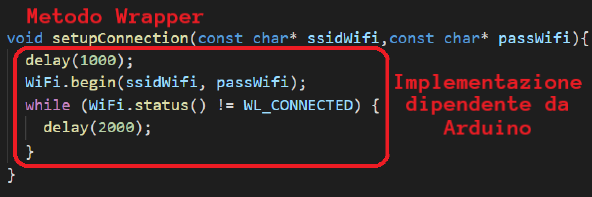
\includegraphics[width=\linewidth]{pics/arduinodependent}
	\caption{Esempio di codice dipendente dalla piattaforma nella classe \texttt{Connection}}
	\label{arduinodep}
\end{figure}

Inoltre, tutte le funzioni specifiche di Arduino utilizzate nel progetto dovranno essere sostituite da funzioni equivalenti per permettere un utilizzo del sistema su dispositivi di tipo PC (ad esempio la funzione \texttt{Serial.print} dovrà essere sostituita da \texttt{cout}).

Nel prossimo capitolo verrà discusso il porting di Edge Engine per dispositivi PC, mantenendo però anche la possibilità di esecuzione su piattaforme Arduino.

\fancypagestyle{plain}{\fancyhead{}\renewcommand{\headrulewidth}{0pt}}
\chapter{Implementazione}
In questa sezione verrà illustrato il porting di Edge Engine da Arduino ESP32 a dispositivi di tipo PC. Al fine di mantenere il prodotto finale slegato dalla piattaforma, si è scelto di utilizzare il compilatore \textbf{g++}, disponibile su dispositivi Windows, Linux e MacOS.\\
In primo luogo verrà discussa l’installazione delle librerie POCO, necessarie per usufruire delle HTTP requests, per poi passare alla modifica del codice preesistente affinché possa essere eseguito sul target desiderato mantenendo però la compatibilità con dispositivi Arduino. In ultimo, verranno mostrati un possibile esempio di utilizzo e la creazione di una libreria vera e propria al fine di permettere una diffusione su più larga scala unita ad una facilità d'uso maggiore.
\section{Librerie POCO}
Come anticipato in precedenza, la prima versione di Edge Engine, in quanto prevista per Arduino, era dotata di due classi wrapper, \textit{Connection} e \textit{APIRest}, adibite alla gestione di risorse hardware e, pertanto, legate alla piattaforma in uso. Di conseguenza, si è resa necessaria la creazione di altre due classi che permettessero di svolgere le stesse funzioni su dispositivi PC. Dal momento che le due classi necessitano di effettuare HTTP requests o di accedere alla rete Internet e l’obbiettivo del progetto è quello di mantenere il più possibile il codice indipentente dalla piattaforma, si è scelto di fare affidamento sulle librerie POCO \cite{POCO}.
\subsection{Installazione}
Le librerie POCO sono un potente strumento C++ multipiattaforma per la creazione di applicazioni basate su rete e Internet che funzionano su desktop, server, dispositivi mobili, IoT e sistemi integrati.\\
L’installazione di queste librerie, tuttavia, si è rivelata più complicata del previsto dal momento che la documentazione riguardante la compilazione delle stesse utilizzando g++ è quasi del tutto assente.\\
\subsubsection{VCPKG, CMake, Conan}
In primo luogo, come da istruzioni del sito POCO, si è tentata l’installazione attraverso il package manager di Windows VCPKG \cite{VCPKG}: un gestore di pacchetti open source multipiattaforma di Microsoft. \\
Nonostante su VCPKG fosse presente il supporto alla compilazione di tali librerie tramite g++, il processo si interrompeva intorno al 70\% a causa del seguente errore:\\
\begin{verbatim}
In file included 
  from C:/mingw/mingw64/x86_64-w64-mingw32/include/mprapi.h:16       
  from C:/mingw/mingw64/x86_64-w64-mingw32/include/iprtrmib.h:12,
  from C:/mingw/mingw64/x86_64-w64-mingw32/include/Iphlpapi.h:15,
  from C:/poco/Foundation/include/Poco/UnWindows.h:33,
  from C:/poco/Foundation/include/Poco/Platform_WIN32.h:22,
  from C:/poco/Foundation/include/Poco/Foundation.h:100,
  from C:/poco/Net/include/Poco/Net/ICMPPacket.h:21,
  from C:\poco\Net\src\ICMPPacket.cpp:15:
C:/poco/Net/include/Poco/Net/ICMPv4PacketImpl.h:72:3: error: 
expected identifier before '(' token
   TIMESTAMP_REQUEST,
   ^~~~~~~~~~~~~~~~~
   
   [...]
   
mingw32-make.exe[2]: *** [Net\CMakeFiles\Net.dir\build.make:679:
Net/CMakeFiles/Net.dir/src/ICMPPacket.cpp.obj] Error 1
mingw32-make.exe[1]: *** [CMakeFiles\Makefile2:530: 
Net/CMakeFiles/Net.dir/all] Error 2
mingw32-make.exe: *** [Makefile:151: all] Error 2

\end{verbatim}
Il secondo tentativo è stato invece effettuato utilizzando CMake \cite{CMake}. CMake è un tool modulare che, con poche e concise istruzioni, è in grado di generare Makefile. CMake dispone di una particolare sintassi comprensiva di moltissime macro ed il loro utilizzo è possibile mediante un apposito file chiamato  \textbf{CMakeLists.txt}. Per la generazione del Makefile e la successiva compilazione del progetto, è necessario eseguire i seguenti comandi:
\begin{verbatim}
mkdir build
cd build
cmake ..
make
\end{verbatim}
Anche in questo caso però, la compilazione si interrompeva attorno al 70\% restituendo lo stesso errore di VCPKG.\\
A seguito dei primi due tentativi falliti, si è scelto di provare a installare le librerie POCO tramite Conan: un package manager open source per lo sviluppo C e C++ che consente ai team di sviluppo di gestire in modo semplice ed efficiente i loro pacchetti e dipendenze tra piattaforme e sistemi di compilazione \cite{Conan}. Il funzionamento di Conan è analogo a quello di VCPKG, ma i file necessari all’installazione delle librerie sono differenti, pertanto ci si sarebbe potuto aspettare un esito differente da quelli passati. Tuttavia, dopo aver seguito le istruzioni specificate dalla guida all'utilizzo, il risultato ottenuto è stato analogo ai precedenti.
\subsubsection{MSYS2}
In ultimo, nonostante non ci fosse alcuna documentazione a riguardo nemmeno sul sito delle librerie POCO, la mancanza di valide alternative ha portato a sperimentare una via differente, rappresentata dal tool MSYS2 \cite{MSYS2}. MSYS2 è una raccolta di strumenti e librerie che fornisce un ambiente di facile utilizzo per la creazione, l'installazione e l'esecuzione di software nativo Windows. Offre build aggiornate per GCC, mingw-w64, CPython, CMake, Meson, OpenSSL, ecc. Per fornire una facile installazione dei pacchetti e un modo per mantenerli aggiornati, è dotato di un package manager chiamato Pacman \cite{Pacman}. Offre molte potenti funzionalità come la risoluzione delle dipendenze e semplici aggiornamenti di sistema, nonché la creazione di pacchetti. La distribuzione del software MSYS2 utilizza un porting di Pacman per creare e gestire (installare, rimuovere e aggiornare) i pacchetti binari.\\
Per poter installare le librerie POCO tramite MSYS2 è necessario eseguire la seguente istruzione sul prompt dei comandi proprietario:
\begin{verbatim}
$ pacman -S mingw64/mingw-w64-x86_64-poco
\end{verbatim}
L’installazione è finalmente riuscita, come è stato possibile verificare tramite i comandi:
\begin{verbatim}
$ pacman -Qi mingw-w64-x86_64-poco
$ pactree mingw-w64-x86_64-poco
\end{verbatim}
Una possibile spiegazione per la quale in questo caso l’installazione sia andata a buon fine potrebbe essere innanzi tutto la differente origine del codice sorgente rispetto ai tool precedentemente utilizzati. Inoltre, come è stato possibile verificare direttamente sulla repository di MSYS2, il package POCO risulta aggiornato pochi giorni prima del tentativo di installazione. Ciò potrebbe indicare una possibile recente risoluzione dei problemi relativi al pacchetto che, probabilmente, non era ancora stata portata a termine nel caso degli altri package manager.
\newpage
\section{Utilizzo}\label{utilizzo}
Per poter usufruire delle librerie POCO precedentemente installate su dispositivi di tipo PC, è necessario seguire alcuni passaggi specifici riguardo le istruzioni da dare al compilatore:
\begin{verbatim}
path\to\mingw64\bin\g++.exe 
-g 
path\to\EdgeEngine_library\examples\EdgineExample.cpp
path\to\EdgeEngine_library\src\connection_windows.cpp
path\to\EdgeEngine_library\src\sample.cpp
path\to\EdgeEngine_library\src\APIRest_windows.cpp
path\to\EdgeEngine_library\src\average.cpp
path\to\EdgeEngine_library\src\edgine.cpp
path\to\EdgeEngine_library\src\filter.cpp
path\to\EdgeEngine_library\src\mapVal.cpp
path\to\EdgeEngine_library\src\maxVal.cpp
path\to\EdgeEngine_library\src\median.cpp
path\to\EdgeEngine_library\src\minVal.cpp
path\to\EdgeEngine_library\src\operation.cpp
path\to\EdgeEngine_library\src\postVal.cpp
path\to\EdgeEngine_library\src\reception.cpp
path\to\EdgeEngine_library\src\script.cpp
path\to\EdgeEngine_library\src\slidingWindow.cpp
path\to\EdgeEngine_library\src\stdDeviation.cpp
path\to\EdgeEngine_library\src\window.cpp
-o
path\to\EdgeEngine_library\examples\CC\EdgeEdgine\EdgineTest.exe
-Ipath\to\msys64\mingw64\include
-Ipath\to\EdgeEngine\edge-engine\EdgeEngine_library\src
-Lpath\to\msys64\mingw64\bin
-Lpath\to\msys64\mingw64\lib
-lPocoFoundation -lPocoUtil -lPocoNet
\end{verbatim}
Come è possibile notare, in assenza di un file \textit{.lib}, è necessario compilare tutte le classi del progetto affinché il proprio main possa funzionare senza errori. Il file di output generato avrà estensione \textit{.exe} e sarà eseguibile da linea di comando.\\
Le ultime cinque righe riguardano invece l'inclusione all'interno del progetto delle librerie POCO. Il comando \textit{-I} è necessario per fornire al compilatore la locazione degli header POCO. \textit{-L}  permette invece di inserire i percorsi aggiuntivi necessari al linker per trovare i file relativi alle librerie. In ultimo, si utilizza il comando \textit{-l} per assegnare al compilatore i nomi delle librerie che sarà necessario linkare.  
\section{Classi wrapper}
Come spiegato in precedenza, la prima versione di Edge Engine è dotata di due classi wrapper che svolgono compiti di connessione alla rete e invio di richieste HTTP, ossia \textit{Connection} e \textit{APIRest}. In questa sezione verrà discusso l’adattamento che si è reso necessario applicare affinché queste due classi potessero essere utilizzate da piattaforme di tipo PC.\\
L’idea iniziale era quella di modificare le classi preesistenti aggiungendo direttive \textit{\#ifdef} che permettessero di passare dalla versione Arduino a quella PC semplicemente definendo una macro. Tuttavia, dal momento che le modifiche da apportare erano troppo invasive, si è preferito creare due nuove classi, \textit{Connection\_windows} e \textit{APIRest\_windows}, che svolgessero lo stesso compito delle due originali, ma per dispositivi di tipo PC. Vedremo in seguito come sia stato reso possibile passare da una piattaforma all'altra tramite il file header \textit{myDefines.h} 
\subsection{Connection\_windows}
La classe \textit{Connection} si occupa unicamente di gestire la connessione WiFi attraverso alcuni metodi che permettono di collegarsi a internet sfruttando la libreria WiFi di Arduino per ESP32. L'istanza di questa classe viene creata nel setup dello sketch e gli unici parametri di cui ha bisogno per stabilire e mantenere la connessione sono le credenziali della rete. Inoltre fornisce metodi utili alla verifica dello stato della connessione e alla riconnessione nel caso in cui questa dovesse venire meno.\\
Nel caso di dispositivi PC, si ha a disposizione un’interfaccia attraverso la quale l’utente può personalmente collegarsi alla rete inserendo le credenziali richieste. Inoltre, stabilire la connessione ad una rete WiFi avrebbe richiesto un’implementazione dipendente dal sistema operativo installato sulla macchina in uso. Pertanto, si è presa la decisione di non implementare i metodi di connessione e riconnessione alla rete, ma soltanto di testarne lo stato. Qualora l’utente non sia connesso a nessuna rete, il programma attenderà finché questo requisito non sarà soddisfatto.\\
In figura \ref{connAW} è mostrato un confronto tra l’implementazione del metodo \textit{isConnected} per Arduino, rispetto a quello per PC.\\
Nel caso Arduino, si può notare come il metodo, al fine di ottenere lo stato della connessione, utilizzi la funzione \textit{WiFi.status} propria della libreria WiFi di Arduino.\\
Nel caso invece dell'implementazione del metodo per PC, siccome utilizzando le librerie POCO non è possibile accedere direttamente allo stato della connessione senza prima effettuare una HTTP request, si è scelto di fare una GET su un sito del quale si avesse certezza di stabilità. Nel caso in cui la richiesta GET non vada a buon fine, si potrà assumere che il dispositivo in uso non sia connesso alla rete Internet.
\begin{figure}[H]
	\centering
	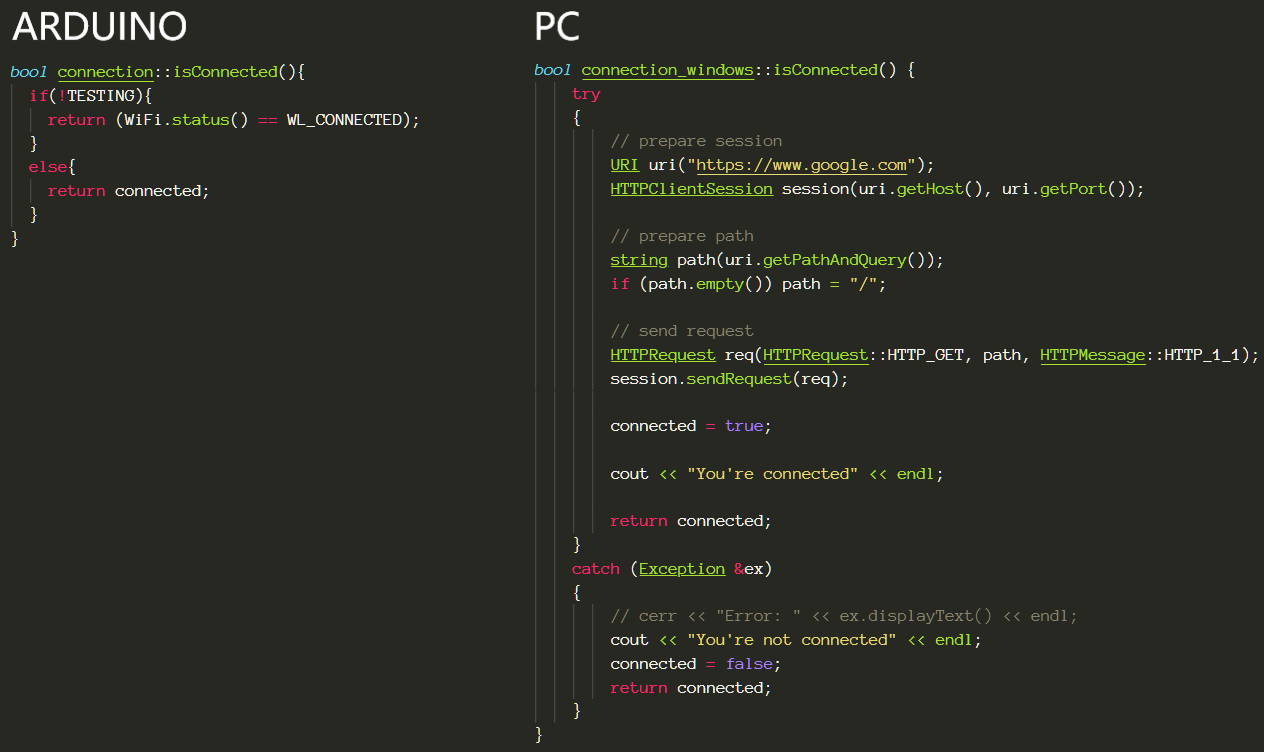
\includegraphics[width=\linewidth]{pics/connAW}
	\caption{Confronto tra le due implementazioni del metodo \textit{isConnected}}
	\label{connAW}
\end{figure}
\subsection{APIRest\_windows}
La classe \textit{APIRest} è un po' più complessa: fornisce un'interfaccia semplificata per l'uso di tutte le richieste HTTP(S) (nel progetto vengono usate solo GET e POST) celando i dettagli della libreria HTTPClient di Arduino. La sua istanza viene utilizzata sia dalla classe principale \textit{edgine} sia dalla classe \textit{postVal}, ultima operazione usata in ogni script che effettua la POST dei dati quando necessario. \textit{APIRest} espone dunque i metodi necessari alla comunicazione con il Cloud occupandosi dei particolari implementativi della piattaforma utilizzata: preparazione dell'header e del body delle richieste, invio e gestione del responso. In seguito al fallimento di una richiesta di informazioni (GET), è l'engine a decidere come comportarsi e se comunicare l'errore al Cloud; se invece a fallire è la trasmissione di un dato o di un issue (POST) allora è questa stessa classe a memorizzare la richiesta fallita e a riprovarne l'invio fino alla corretta ricezione da parte del Cloud. Per ragioni principalmente energetiche questi tentativi vengono fatti ogni qualvolta si renda necessario effettuare l'invio di un nuovo dato e non in maniera continuativa.\\
In ultimo tale classe ha il compito di calcolare e fornire la data e l'ora correnti da allegare alle misurazioni e alle comunicazioni d'errore.\\
Dal momento che \textit{APIRest} fa largo uso della libreria HTTPClient di Arduino, si è resa necessaria una nuova implementazione della stessa per dispositivi PC, \textit{APIRest\_windows}. Questa classe ha il compito di svolgere le stesse funzioni dell’originale, ma, in questo caso, avvalendosi delle librerie POCO, al fine di rispettare le specifiche di compatibilità con altre piattaforme. In figura \ref{APIRestAW} è possibile notare le differenti implementazioni della funzione \textit{POSTLogin}, adibita all'autenticazione sul Cloud e alla successiva ricezione del JWT.\\
\begin{figure}[H]
	\centering
	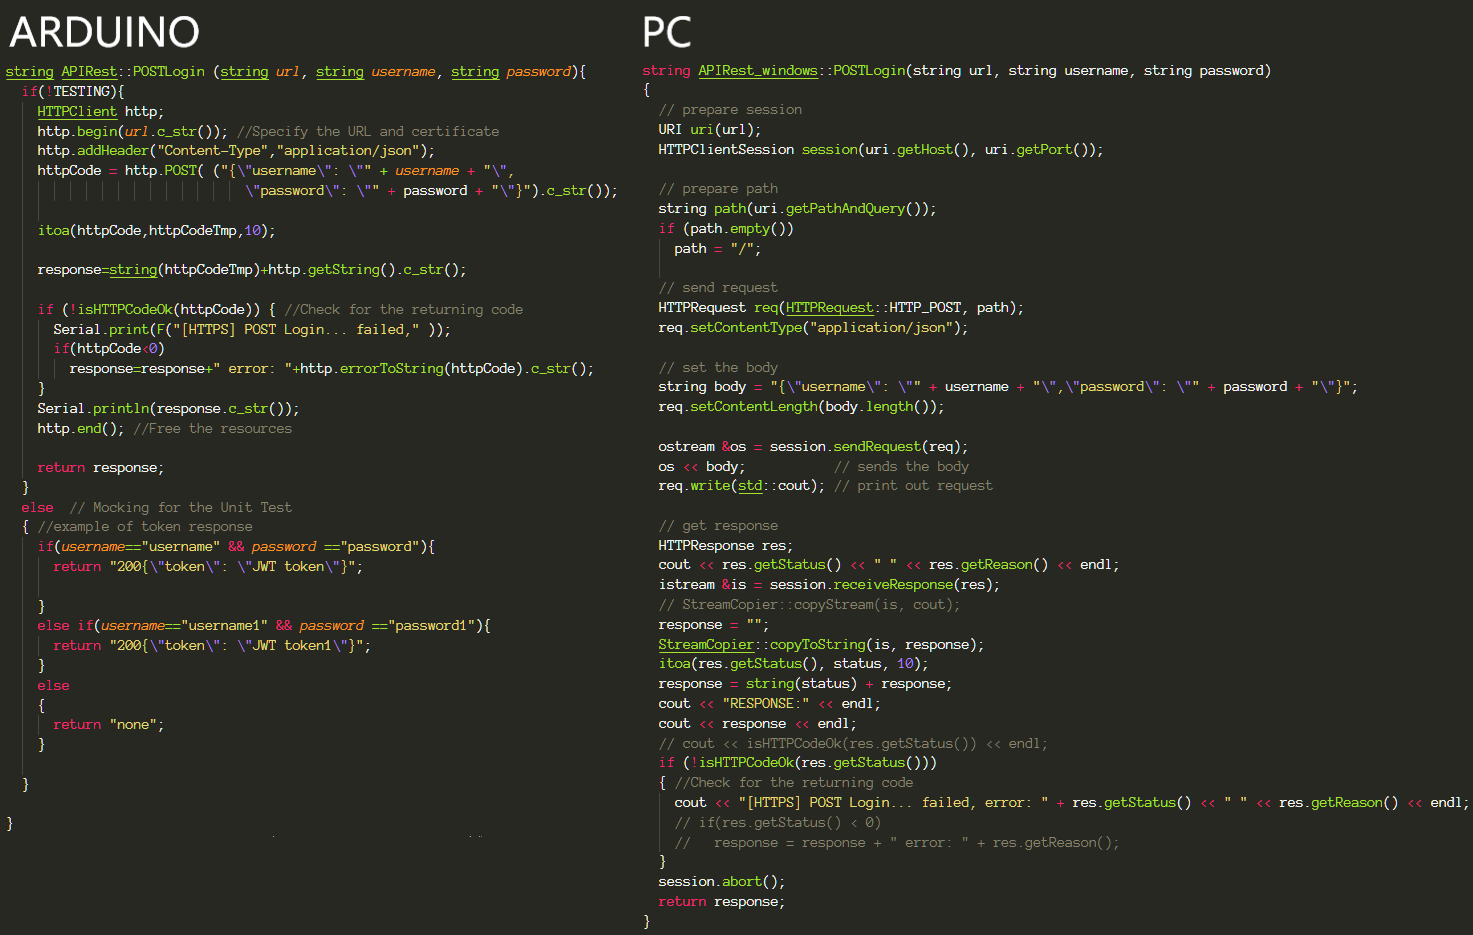
\includegraphics[width=\linewidth]{pics/APIRestAW}
	\caption{Confronto tra le due implementazioni del metodo \textit{PostLogin}}
	\label{APIRestAW}
\end{figure}
In primo luogo, il metodo prende in ingresso tre stringhe: url del server, username e password dell'utente necessari ad ottenere i permessi per accedere alle proprie risorse. In seguito viene eseguita una POST all'interno del cui \textit{body} vengono specificati username e password, scritti in formato JSON. La \textit{response} conterrà lo stato della richiesta HTTP, che indica se l'operazione sia andata a buon fine o meno, e il JWT necessario per gli accessi futuri alle risorse.
\subsection{myDefines.h}
\begin{wrapfigure}{r}{6cm}
	\centering
	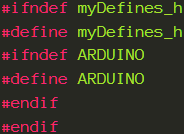
\includegraphics{pics/myDefines}
	\caption{myDefines.h}
	\label{myDefines}
\end{wrapfigure}
Una volta implementate le due classi wrapper \textit{Connection\_windows} e \textit{APIRest\_windows}, volendo mantenere la possibilità di passare da una piattaforma all'altra in modo rapido e semplice, si è scelto di creare un header file, \textit{myDefines.h}, attraverso il quale fosse possibile decidere il target di esecuzione del proprio codice senza necessità di modificare ulteriori files. \textit{myDefines.h} ha la struttura mostrata in figura \ref{myDefines}.
Essa consiste semplicemente nella definizione della macro \textit{ARDUINO} nel caso in cui si desideri compilare per tale piattaforma. Laddove invece tale macro non fosse definita, verrebbe scelta di default la compilazione per PC. \textit{myDefines.h}, dovrà essere inclusa in tutti i file che utilizzano i metodi delle classi wrapper sopra descritte. All'interno di tali file, lo switch di piattaforma è gestito tramite direttive \textit{ifdef}, come visibile in figura \ref{ifdef}.
\begin{figure}[H]
	\centering
	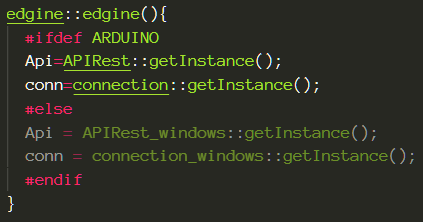
\includegraphics[width=0.66\linewidth]{pics/ifdef}
	\caption{Esempio di utilizzo della direttiva \textit{ifdef}}
	\label{ifdef}
\end{figure}
In questa specifica situazione, nel caso in cui, come in figura, sia definita la macro \textit{ARDUINO}, verranno create istanze delle classi \textit{Connection} e \textit{APIRest}, altrimenti delle classi \textit{Connection\_windows} e \textit{APIRest\_windows}.
\section{Esempio di prova}\label{prova}
Dopo aver ultimato l’implementazione delle classi citate in precedenza, si è deciso di sviluppare un semplice \textit{main} per PC che simulasse un’applicazione IoT per il monitoraggio della temperatura, al fine di testare quanto realizzato.\\
Il device simulato possiede una feature: temperature. In prima istanza è necessario impostare tutti i parametri della descrizione virtuale e creare all'interno del Cloud la risorsa che rappresenti il dispositivo d’interesse. Dopodiché bisogna costruire gli scripts che si intende eseguire sui flussi di dati e assegnarli alla risorsa precedentemente creata sulle API di tale dispositivo. È necessario inoltre creare un utente (parametri username e password nel codice) sul Cloud attraverso il quale l'engine potrà autenticarsi.\\
Il \textit{main} è suddiviso in due fasi principali, associate alle funzioni  \textit{setup} e  \textit{loop} che richiamano la configurazione tipica degli sketch Arduino. Le procedure da svolgere nella funzione  \textit{setup} sono la configurazione del sensore, l'avvio della connessione Internet e l'assegnazione dei parametri alla struttura dati \textit{options} per inizializzare l'engine. Nella funzione \textit{loop} invece, è disposta la creazione dei sample (connotati da features, data e valore letto dai sensori), poi processati dall'engine tramite gli script ricevuti dal Cloud. Tali script vengono eseguiti ciclicamente e il risultato delle operazioni portate a termine viene conservato sul Cloud. Il processo di interazione Cloud-Edge appena descritto è riassunto nella tabella \ref{loop}. In questo specifico caso, siccome si tratta di un esempio di test e non di un'applicazione reale, la funzione \textit{loop} viene eseguita una volta sola, dal momento che l'interesse non è l'invio dei dati in maniera iterativa, ma di verificare il funzionamento di un singolo script.\\
Già da un esempio semplice come quello appena descritto, ci si può rendere conto di come la realizzazione di un'applicazione IoT servendosi di Edge Engine riduca in maniera drastica la quantità di codice da produrre e il tempo di sviluppo del software. Esso fornisce la possibilità non solo di eseguire in locale gli scripts caricati da remoto, ma anche di inviare e ricevere delle informazioni dal Cloud e gestire eventuali malfunzionamenti comunicandone l'avvenimento al server online.
\begin{table}[H]
	\centering
	\begin{tabular}{|l|l|l|}
		\hline
		\textbf{Request} & \textbf{Task} & \textbf{Descrizione}\\
		\hline
		\textbf{POST} & Credenziali di Login & Viene ricevuto il JWT dal Cloud\\
		\hline
		\textbf{GET} & Descrizione del device & Gli script vengono recuperati dal Cloud\\
		\hline
		\textbf{POST} & Measurements & I dati vengono salvati sul Cloud\\	
		\hline
	\end{tabular}
	\caption{Le HTTP requests generalmente eseguite da Edge Engine}
	\label{loop}
\end{table}
\section{Creazione della libreria}
Come è stato possibile notare nella sezione \ref{utilizzo}, il sistema, per poter essere utilizzato, necessita della compilazione di tutte le classi del progetto, andando dunque a rendere obbligatoria anche la presenza dei file \textit{.cpp} oltre agli header all'interno del proprio ambiente di sviluppo. Questa procedura è assai utile in fase di sviluppo del sistema, dal momento che in questo modo è possibile agire direttamente sulle classi in caso di errori o necessità di cambiamenti al codice. Tuttavia, non lo è altrettanto nel caso di utilizzo dell'Edge Engine da parte di sviluppatori che desiderino farne uso senza volontà di applicare modifiche al codice sorgente o qualora si desideri che la propria implementazione dei vari metodi non sia visibile a chi ne usufruisce.\\
Di conseguenza, si è deciso di creare un file \textit{.lib} grazie al quale è facilitata la fruizione del sistema da parte di altri sviluppatori e, al contempo, viene nascosta la realizzazione relativa alle classi appartenenti al progetto.\\
Di seguito vengono mostrati i passaggi che è necessario eseguire per ottenere il file \textit{.lib} a partire dal codice sorgente:
\begin{verbatim}
g++ -c APIRest_windows.cpp 
      -Ipath\to\EdgeEngine_library\src 
      -Ipath\to\msys64\mingw64\include 
g++ -c connection_windows.cpp 
      -Ipath\to\EdgeEngine_library\src 
      -Ipath\to\msys64\mingw64\include 

[...]

g++ -c window.cpp
      -Ipath\to\EdgeEngine_library\src 
      -Ipath\to\msys64\mingw64\include 
 
ar rcs Edgine.lib APIRest_windows.o connection_windows.o [...] 
      window.o
\end{verbatim}
I primi passaggi, da ripetere per ogni classe presente all'interno del progetto, producono per ognuna il relativo file in formato \textit{.o}, necessario per la successiva creazione del \textit{.lib}. Il comando \textit{ar} poi, a partire da i file \textit{.o} appena creati, genera la libreria \textit{Edgine.lib}.\\
Infine, per poterla utilizzare all'interno del proprio progetto, sono necessarie le seguenti direttive per il compilatore:
\begin{verbatim}
-g
main.cpp
-o
main.exe
-Ipath\to\library\repository\include
-Ipath\to\msys64\mingw64\include
-Lpath\to\library\repository\lib
-Lpath\to\msys64\mingw64\lib
-lEdgine
-lPocoFoundation
-lPocoUtil
-lPocoNet
\end{verbatim}









\fancypagestyle{plain}{\fancyhead{}\renewcommand{\headrulewidth}{0pt}}
\chapter{Esperimenti}
Una volta ultimata l’implementazione del codice, ora più facilmente fruibile grazie alla creazione del file \texttt{.lib}, il passo successivo è stato lo sviluppo di applicazioni vere e proprie che potessero fare affidamento sulla libreria Edge Engine. In particolare, in questo capitolo verranno trattati tre esperimenti differenti: il primo riguarderà un esempio di utilizzo su PC Windows (più completo e significativo rispetto a quello descritto nella sezione \ref{prova}, il secondo verterà invece sulla creazione di un plugin per poter usufruire della libreria anche in ambiente Unity3D e, infine, il terzo descriverà un vero e proprio caso applicativo portato a termine da due tesisti triennali del corso di Ingegneria Elettronica e Tecnologie dell'Informazione dell'Università degli Studi di Genova.
\section{Applicazione Windows}
L'esempio di utilizzo per Windows è stato creato al fine di mostrare e testare tutte le potenzialità offerte dall'incremento delle piattaforme supportate da Edge Engine.

Come accennato brevemente nella sezione \ref{prova}, in primo luogo è necessario riportare sul Cloud la descrizione della risorsa che si intende adottare. Più in particolare, sono da specificare i parametri mostrati nella tabella seguente:

\begin{table}[H]
	\begin{tabular}{|p{0.15\textwidth}|p{0.44\textwidth}|p{0.32\textwidth}|}
		\hline
		\textbf{Parametri} & \textbf{Nome} & \textbf{URL}\\
		\hline
		\textbf{Thing} & my-pc & {{url}}/v1/things/my-pc\\
		\hline
		\textbf{Feature} & total-ram, total-rom, available-ram, available-rom & {{url}}/v1/features\\
		\hline
		\textbf{Device} & pc-probe & {{url}}/v1/devices/pc-probe\\	
		\hline
		\textbf{Script} & total-rom-installed, total-ram-installed, ram-available, rom-available, average-hourly-available-ram, ram-available-to-mb, rom-available-to-mb,  max-available-ram, max-available-rom & {{url}}/v1/scripts\\	
		\hline
	\end{tabular}
\\\\url = \url{http://students.atmosphere.tools/}
	\caption{Parametri Measurify della risorsa Windows}
	\label{paramMeas}
\end{table}

Il device \texttt{pc-probe} contiene all'interno della sua descrizione le features e gli script ad esso associati. Le prime indicano le grandezze fisiche misurabili dal dispositivo, mentre i secondi rappresentano le funzioni di elaborazione che è possibile applicare ai dati ricevuti. 

La tabella \ref{script} mostra la struttura degli script implementati. Essi sono composti da due campi principali: \texttt{\_id} e \texttt{code}.  \texttt{\_id} specifica il nome associato allo script stesso, mentre \texttt{code} contiene le effettive operazione che il dispositivo fisico andrà ad effettuare. 

\begin{table}[H]
	\begin{tabular}{|p{0.27\textwidth}|p{0.67\textwidth}|}
		\hline
		\textbf{\_id} & \textbf{code} \\
		\hline
		ram-available & available-ram().send()\\
		\hline
		rom-available & available-rom().send()\\
		\hline
		total-ram-installed & total-ram().send()\\
		\hline
		total-rom-installed & total-rom().send()\\
		\hline
		max-available-ram & available-ram(10).max().send()\\	
		\hline
		max-available-rom & available-rom(10).max().send()\\
		\hline	
		ram-available-to-mb & available-ram().map(a*1024).send()\\
		\hline
		rom-available-to-mb & available-rom().map(a*1024).send()\\
		\hline
		average-hourly-available-ram & available-ram(6m).window(+,0,10).map(a/10).send()\\
		\hline
	\end{tabular}
	\caption{Script correlati al device \texttt{pc-probe}}
	\label{script}
\end{table}

Prendendo ad esempio lo script \texttt{ram-available-to-mb}, il codice in oggetto permette di ricavare la quantità, espressa in gigabyte, di memoria disponibile tramite l’operazione \texttt{available-ram()}, la quale viene poi concatenata a \texttt{map(a*1024)} che converte il valore ottenuto in megabyte moltiplicandolo per 1024. Infine, tramite la \texttt{send()} il campione appena elaborato viene inviato a Measurify.

Lo script \texttt{average-hourly-available-ram}, invece, calcola la media oraria di ram disponibile, ma necessita di un tempo di elaborazione più lungo di una singola esecuzione dell'engine, come specificato dal codice:\\ \texttt{available-ram(6m).window(+,0,10).map(a/10).send()}\\ L’operazione \texttt{available-ram(6m)} permette di campionare ogni sei minuti. Tramite la \texttt{window(+,0,10)} poi, viene presa una finestra di dieci input e calcolata la somma di tali elementi. Il calcolo della media viene poi portato a termine grazie alla \texttt{map(a/10)}, che opera una divisione sul totale per il numero di campioni presi in considerazione. Infine, il risultato viene inviato al Cloud grazie alla \texttt{send()}.

Una volta riportata sul Cloud la descrizione della risorsa di cui si intende usufruire, è possibile passare allo sviluppo del codice dell'applicazione. Si hanno nuovamente due funzioni principali, \texttt{setup} e \texttt{action}, che svolgono gli stessi task di autenticazione, elaborazione e invio dei dati descritti nella sezione \ref{prova}. In questo caso però, \texttt{action} viene eseguita ciclicamente per un numero di volte specificato dalla variabile \texttt{loopCount}. Questo al fine di poter disporre di un tempo di esecuzione più lungo, nel caso in cui si desideri, ad esempio, usufruire dello script \texttt{average-hourly-available-ram}, il quale richiede un'ora di tempo per collezionare i campioni.

Inoltre, al fine di recuperare dalla macchina in uso le informazioni relative all'utilizzo delle memorie RAM e ROM, sono state implementate le funzioni \texttt{getRAMinfo} e  \texttt{getROMinfo}. Esse sono esclusive per piattaforme dotate di sistema operativo Windows in quanto fanno uso della libreria proprietaria. Qualora si riveli necessario modificare il progetto al fine di adattarlo ad altri OS, sarà sufficiente sostituire le suddette funzioni con altre, specifiche del target desiderato.

Un esempio di dato elaborato dallo script \texttt{ram-available-to-mb} del device \texttt{my-pc} e conservato sul Cloud è mostrato in figura \ref{datowin}.

\begin{figure}[H]
	\centering
	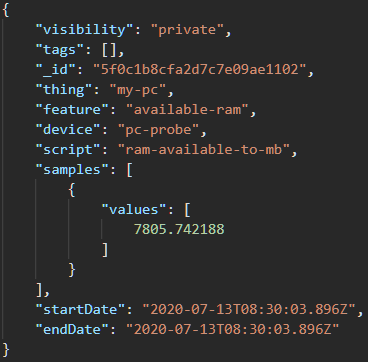
\includegraphics[scale=0.7]{pics/datowin}
	\caption{Dato relativo al valore di memoria RAM disponibile convertito in MB e conservato sul Cloud}
	\label{datowin}
\end{figure}

\section{Applicazione alla Realtà Virtuale}
Edge Engine nasce con l’idea di offrire uno strumento modulare e slegato dall'hardware che possa facilitare e incentivare lo sviluppo di applicazioni IoT. Questo motore, oltre ad essere una valida soluzione per tale scopo, potrebbe inoltre risultare ugualmente efficace in un contesto totalmente differente, come quello dei videogiochi. Ciò è dovuto al fatto che, attualmente, non esiste uno strumento che elabori al tempo stesso dati provenienti da sorgenti così eterogenee come possono essere un sensore fisico ed uno presente all'interno di un mondo virtuale. Si pensi ad esempio ad un videogiocatore che abbia intenzione di monitorare il proprio battito cardiaco e, al contempo, processare dati provenienti dall’ambiente di gioco. Edge Engine, se adattato ad un Integrated Development Environment (IDE) dedito alla creazione di videogiochi, potrebbe essere in grado di svolgere entrambi i task richiesti grazie all’alto livello di scalabilità di cui dispone.

Come ultimo obiettivo, dunque, si intende trattare lo sviluppo di un’applicazione per Unity3D in modo da poter osservare il funzionamento di Edge Engine in un contesto, la realtà virtuale, diverso da quello per cui era stato inizialmente pensato, ma che può spesso rivelarsi strettamente collegato, o collegabile, all'ambiente reale.

In primo luogo verranno descritti i passi richiesti per la creazione di un plugin, necessario al fine di utilizzare Edge Engine all'interno dell'ambiente Unity3D. In seconda istanza poi, sarà discussa l'implementazione di un'applicazione di esempio che sfrutti il plugin in precedenza sviluppato.
\subsection{Plugin}\label{plugin}
All'interno di Unity, normalmente si utilizzano gli script C\# per creare funzionalità, ma è anche possibile includere codice creato al di fuori di Unity sotto forma di plugin. I plugin sono librerie di codice nativo specifiche della piattaforma. Possono accedere a funzionalità come chiamate del sistema operativo e librerie di codici di terze parti che altrimenti non sarebbero disponibili per Unity. Tuttavia, queste librerie non sono accessibili agli strumenti di Unity come le normali librerie utilizzabili all'interno dell'IDE.

Per la creazione del plugin, che corrisponde in tutto e per tutto ad una dynamic-link library (DLL), si è scelto di utilizzare Visual Studio, data l'affinità di tale IDE con Unity. Dal momento che il compilatore offerto da Visual Studio, MSVC, è differente da g++, usato in precedenza per la creazione della libreria Edge Engine e l’installazione delle librerie POCO, è stato in primo luogo necessario ricompilare entrambi i progetti.

Per quanto riguarda le librerie POCO, in questo caso, siccome il compilatore proposto di default da VCPKG è proprio MSVC, in quanto sviluppati entrambi da Microsoft, si è deciso di utilizzare questo package manager, scegliendo la versione a 64 bit. Rispetto ai problemi riscontrati in precedenza con il compilatore g++, l’installazione delle librerie è andata a buon fine senza intoppi. Per la compilazione è necessario eseguire i seguenti comandi:

\begin{verbatim}
vcpkg install poco:x64-windows
vcpkg integrate install
\end{verbatim}

Il comando di \texttt{integrate install} non è obbligatorio, ma semplifica l'utilizzo delle librerie POCO all'interno dei progetti, evitando allo sviluppatore di dover inserire le locazioni degli header e dei file \texttt{.lib}, necessari alla compilazione.

Per quanto riguarda invece la libreria Edge Engine, è stato creato nuovamente un file \texttt{.lib}, ma questa volta, facendo affidamento a MSVC per i motivi sopracitati. Per poter poi utilizzare tale libreria all'interno del progetto di creazione della DLL, è stato necessario fornire al compilatore, tramite la schermata di impostazioni di Visual Studio, la locazione degli header e del file \texttt{Edgine.lib}.

Dopo aver messo le basi per la creazione della libreria dinamica che verrà poi utilizzata come plugin all'interno di Unity, è possibile passare alla fase di implementazione della stessa.

Lo schema della DLL che è stata prodotta prevede una singola classe, dentro la quale sono presenti le funzioni a cui si intenderà poi fare riferimento dal lato C\#, e il relativo header. All'interno di quest'ultimo è necessario definire tali funzioni con l’attributo \texttt{\_\_declspec(dllexport)}, il quale indica che esse potranno essere chiamate dallo script che sfrutta il plugin. Inoltre, tramite la keyword \texttt{extern "C"}, si indica al compilatore che le funzioni in oggetto devono impiegare la convenzione di linking del linguaggio C. Ciò è necessario al fine di esportarle correttamente, altrimenti, a causa del mangling operato dai compilatori C++, non sarebbe poi possibile far riferimento ad esse in ambiente Unity. Il mangling è una tecnica utilizzata per distinguere funzioni che hanno lo stesso nome (overloading). Essa consiste nella manipolazione del nome in fase di compilazione affinché esso sia univoco, ma, in questo specifico caso, ciò renderebbe ignoto allo sviluppatore il nome definitivo associato e, per questo motivo, non sarebbe in grado di utilizzare tali funzioni all'interno del plugin. Il linguaggio C, invece, non prevede il mangling delle funzioni, dal momento che la tecnica di overload non è supportata. Pertanto, il file binario generato dalla compilazione conterrà i nomi originali delle funzioni esportate, che potranno essere chiamate dal lato C\# senza incongruenze. Siccome la convenzione di linking adottata è quella del linguaggio C, è necessario che, nonostante il corpo delle funzioni sia scritto in C++, i tipi di dato di input e output debbano essere quelli propri del C.

Andando, come di consueto, a riprendere la struttura degli sketch Arduino, si è scelto di implementare due funzioni esportabili: \texttt{Setup} e \texttt{Action}. Il loro funzionamento è analogo ai casi precedentemente discussi, con un’importante differenza relativa all’inserimento delle caratteristiche descrittive quali \textit{device}, \textit{thing}, \textit{feature}, \textit{username} e \textit{password}. In questo specifico caso infatti, se prima tali informazioni era necessario inserirle all'interno del codice, si è scelto di renderle configurabili da parte dell'utente dal lato Unity. Di seguito sono mostrate le firme delle due funzioni in oggetto:

\begin{verbatim}
void Setup(char* myId, char* myPw, char* myThing, char* myDevice,
           char* myDeviceId)
void Action(char* sampleName, float hits)
\end{verbatim}

La \texttt{Setup} prende in ingresso nell'ordine \textit{username}, \textit{password}, \textit{thing}, \textit{device}  e \textit{deviceId}, un identificativo univoco per ogni dispositivo.

La \texttt{Action}, invece, riceve il nome della \textit{feature} e il relativo dato misurato per poterlo processare e inviare successivamente al Cloud.

Il progetto così compilato produce i file \texttt{NATIVECPPLIBRARY.dll}, \\\texttt{pcred.dll}, \texttt{PocoFoundationd.dll}, \texttt{PocoNetd.dll}, \texttt{zlibd1.dll}. Il primo rappresenta proprio la libreria dinamica contenente le funzioni appena create che verranno poi utilizzate all'interno di uno script Unity. Il secondo, invece, è una DLL di file si sistema essenziali dell'OS Windows. Infine, gli ultimi tre sono un’elaborazione, operata durante la creazione della DLL, delle librerie POCO, necessarie al funzionamento di  \texttt{NATIVECPPLIBRARY.dll}. Al fine di utilizzare all'interno di Unity la DLL appena creata, è necessario copiare questi files dentro la cartella di progetto.
\subsection{Unity}

\begin{figure}[H]
	\centering
	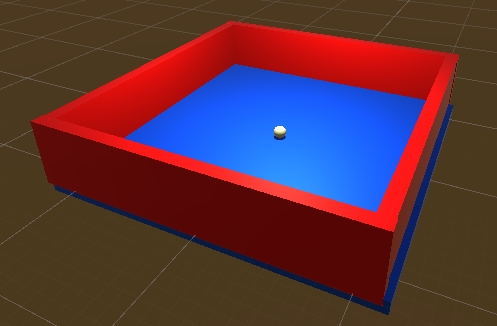
\includegraphics[scale=1.1]{pics/ring}
	\caption{Scena di gioco Unity3D}
	\label{ring}
\end{figure}

Sul fronte Unity, avendo come obbiettivo primario il test delle funzionalità di Edge Engine anche in un contesto di realtà virtuale, si è deciso di creare una semplice applicazione di esempio che potesse essere in grado di raccogliere dati provenienti dalla scena di gioco e, tramite il plugin descritto precedentemente, di inviarli a Measurify. In particolare, è stato creato un ring contenente al suo interno una pallina controllabile tramite i tasti freccia del PC (si veda fig. \ref{ring}). Ogniqualvolta la pallina urta uno dei quattro muri delimitanti, la collisione viene registrata all'interno di una variabile incrementale e, in caso di raggiungimento di un numero di collisioni che sia multiplo di cinque (lo zero è escluso per ovvi motivi), tale valore viene inviato al Cloud. Come si può facilmente dedurre, tale applicazione, differentemente da quella per Windows, rappresenta un mero esempio di utilizzo di Edge Engine all'interno dell'ambiente di gioco e non intende in alcun modo mostrare un vero e proprio caso applicativo, dal momento che non è questo lo scopo del progetto Unity.

In primo luogo è stato necessario inserire la descrizione della risorsa all'interno di Measurify, riassunta in tabella \ref{descunitydev}.

\begin{table}[H]
	\begin{tabular}{|p{0.15\textwidth}|p{0.30\textwidth}|p{0.46\textwidth}|}
		\hline
		\textbf{Parametri} & \textbf{Nome} & \textbf{URL}\\
		\hline
		\textbf{Thing} & ball & {{url}}/v1/things/ball\\
		\hline
		\textbf{Feature} & collision & {{url}}/v1/features/collision\\
		\hline
		\textbf{Device} & unityDevice & {{url}}/v1/devices/unityDevice\\	
		\hline
		\textbf{Script} & collisions-count-send & {{url}}/v1/scripts/collisions-count-send\\	
		\hline
	\end{tabular}
	\\\\url = \url{http://students.atmosphere.tools/}
	\caption{Parametri Measurify della risorsa Unity}
	\label{descunitydev}
\end{table}

Come spiegato in precedenza, siccome quest'applicazione è pensata per essere un semplice esempio guida, il valore associato alla sola feature \texttt{collision} viene inviato così com'è, senza alcuna elaborazione intermedia.

Veniamo dunque allo sviluppo dello script C\# che permette la fruizione della libreria Edge Engine anche all'interno di Unity.  

\begin{wrapfigure}{r}{7.5cm}
	\centering
	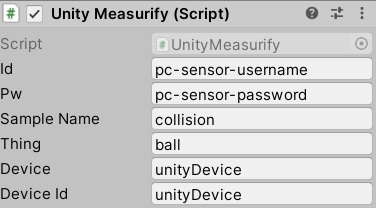
\includegraphics[scale=0.85]{pics/unityscriptvars}
	\caption{\centering{Variabili settabili dall'utente all'interno dell'inspector Unity}}
	\label{unityscriptvars}
\end{wrapfigure}

Ricordando la struttura delle funzioni esportate dal plugin mostrata nella sezione \ref{plugin}, le quali prevedono di ricevere in ingresso i nomi dei parametri descrittivi della risorsa, oltre alle credenziali di accesso, al fine di mantenere un elevato livello di configurabilità si è scelto di impostare queste variabili come settabili da parte dell'utente dichiarandole \texttt{public}, come visibile in figura \ref{unityscriptvars}. Così facendo lo sviluppatore sarà poi in grado di personalizzare a proprio piacimento i dettagli relativi al proprio caso applicativo.

Successivamente, per poter far uso all'interno di Unity delle funzioni \texttt{Setup} e \texttt{Action}, esposte dal plugin, è necessario dichiararle con l’attributo \texttt{DLLImport}, come mostrato di seguito:

\begin{verbatim}
[DllImport("NATIVECPPLIBRARY", EntryPoint = "Setup")]
public static extern void Setup(StringBuilder myId, 
            StringBuilder myPw, StringBuilder myThing, 
            StringBuilder myDevice, StringBuilder myDeviceId);

[DllImport("NATIVECPPLIBRARY", EntryPoint = "Action")]
public static extern void Action(StringBuilder mySample, 
            float data);
\end{verbatim}

\begin{itemize}
	\item \texttt{DLLImport} indica l'importazione da una DLL;
	\item \texttt{EntryPoint} fornisce al compilatore il nome che la funzione ha all'interno del plugin;
	\item \texttt{extern} è un attributo necessario per dichiarare una funzione che è implementata esternamente.
\end{itemize}

Come è possibile notare, il passaggio dei parametri testuali avviene per lo più attraverso dati di tipo \texttt{StringBuilder}. Ciò è dovuto al fatto che l’utilizzo della memoria di \texttt{StringBuilder} e array di \texttt{char} è simile, pertanto il plugin è in grado di interpretare correttamente il contenuto del primo definito dal lato Unity. 

Come di consueto, lo script Unity è organizzato nel seguente modo: un metodo \texttt{Start}, che viene eseguito una sola volta all’avvio del programma, e uno, \texttt{Update}, che viene invece ripetuto ciclicamente. Dal momento che, anche in questo caso, lo schema di base è simile a quello degli sketch Arduino, va da sé che la funzione \texttt{Setup} verrà chiamata all'interno di \texttt{Start}, mentre la \texttt{Action} dentro \texttt{Update}, come visibile in figura \ref{startupdate}. 

\begin{figure}[H]
	\centering
	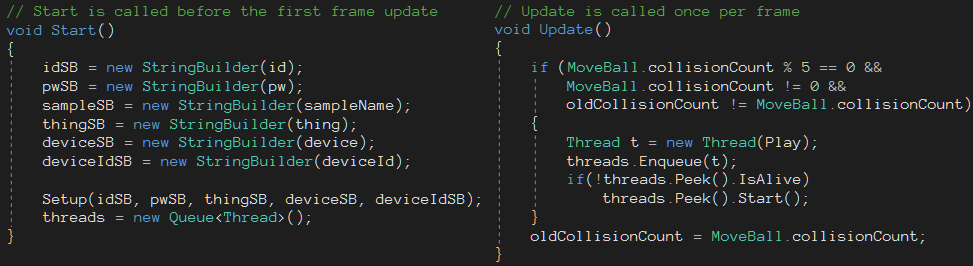
\includegraphics[width=\linewidth]{pics/startupdate}
	\caption{Metodi \texttt{Start} e \texttt{Update} dello script Unity}
	\label{startupdate}
\end{figure}

\texttt{Start} ha il compito di inizializzare tutte le variabili pubbliche di tipo \texttt{StringBuilder} coinvolte nello script. Una volta recuperati i parametri inseriti dall'utente, viene eseguita la \texttt{Setup} che, si rammenta, permette di autenticarsi su Measurify ottenendo il JWT per gli accessi successivi. In ultimo, viene inizializzato un oggetto di tipo \texttt{Queue<Thread>} che si occuperà di gestire le future chiamate della funzione \texttt{Action}. La creazione di oggetti di tipo \texttt{Thread} è necessaria in quanto, altrimenti, la normale esecuzione del programma verrebbe interrotta per qualche istante ad ogni invio dei dati al Cloud, a causa del tempo necessario a compiere questo task. Grazie all'utilizzo dei thread, l'applicazione potrà continuare il suo normale svolgimento mentre, in parallelo, la funzione \texttt{Action} viene portata a termine. I thread vengono inseriti all'interno di una coda al fine di ottenere una più semplice gestione degli stessi, avendo la possibilità di crearli, eseguirli e distruggerli in modo ordinato facendo uso dei metodi \texttt{Enqueue}, \texttt{Peek} e \texttt{Dequeue}.

\texttt{Update}, innanzitutto, esegue un controllo relativo al numero di collisioni che la pallina ha effettuato. Tale valore deve essere multiplo di cinque, diverso da zero e differente dal dato precedentemente inviato al Cloud in modo da non avere duplicati. Se queste tre condizioni sono soddisfatte, viene creato un nuovo thread e aggiunto alla coda. Qualora il programma non ne stia già eseguendo uno precedentemente creato, il thread viene eseguito. Tutti quelli rimasti nella coda alla chiusura dell'applicazione saranno lanciati, prima dell'effettivo termine del programma, dal metodo \texttt{OnApplicationQuit}. In questo modo l'applicazione, a regime, non è sovraccarica di un eccessivo numero di thread e, al contempo, viene garantita l'esecuzione di ciascuno di essi entro la conclusione del programma, momento in cui l'utente non interagisce più con la scena di gioco.

Dall'immagine mostrata in figura \ref{risorsaunity} si può notare come, grazie alla creazione del plugin e all'implementazione di uno script che sfrutta tale DLL, Edge Engine sia ora in grado di comunicare correttamente con Measurify anche quando utilizzato in un contesto di realtà virtuale.

\begin{figure}[H]
	\centering
	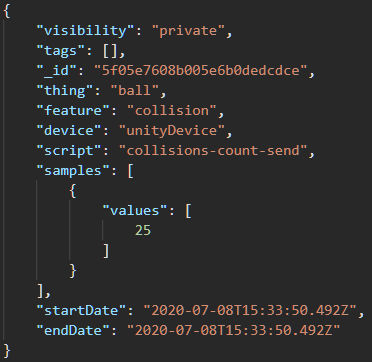
\includegraphics[scale=0.7]{pics/measunity}
	\caption{Dato relativo al numero di collisioni effettuate dalla pallina conservato sul Cloud}
	\label{risorsaunity}
\end{figure}

\subsection{Applicazione reale}
Questa sezione, diversamente da quelle precedenti, non riguarda l’implementazione di Edge Engine su nuove piattaforme, bensì l’utilizzo di tale sistema da parte di due tesisti triennali. In particolare, il progetto in questione tratta di un rilevatore di movimento, composto da un sensore PIR HC-SR501 installato su scheda Arduino ESP8266, il quale necessita di comunicare con il Cloud Measurify per potervi inviare i dati registrati dall'ambiente circostante (si veda fig. \ref{esp8266cloud}). Le potenzialità offerte da Edge Engine risultano adatte allo sviluppo di un’applicazione del genere, siccome la gestione delle HTTP requests viene interamente gestita dall'engine permettendo dunque agli sviluppatori di adoperarsi maggiormente sugli aspetti di collegamento sensore - board.

\begin{figure}[H]
	\centering
	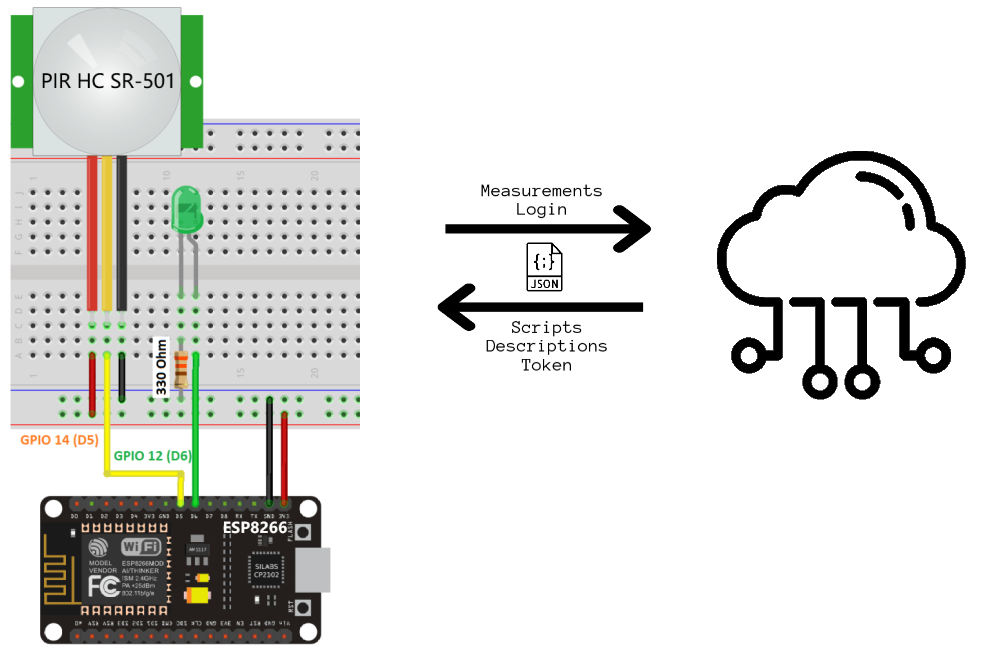
\includegraphics[width=\linewidth]{pics/esp8266cloud}
	\caption{Schema funzionale di Edge Engine per Arduino}
	\label{esp8266cloud}
\end{figure}

Riguardo proprio la comunicazione tra sensore e board, che avviene tramite Interrupt Service Routine (ISR), si è resa peraltro necessaria una piccola modifica al codice sorgente di Edge Engine. In particolare, nella funzione \texttt{getActualDate} della classe \texttt{APIRest}, chiamata proprio all'interno della ISR, veniva definita una variabile di tipo \texttt{float}. Tuttavia, l'utilizzo di tale tipologia di dato all'interno degli interrupt causa la seguente eccezione del coprocessore:

\begin{verbatim}
Guru Meditation Error: 
          Core 1 panic'ed (Coprocessor exception [...])
\end{verbatim}

Ciò è dovuto all'intervento della Floating-Point Unit (FPU), non supportata all'interno della ISR. Pertanto, la soluzione adottata è stata la sostituzione del tipo \texttt{float} con \texttt{long} che, non essendo a virgola mobile, non presenta questa problematica.

Come previsto, i benefici riscontrati dall'utilizzo di Edge Engine, a detta dei diretti interessati,  sono stati molteplici. In primo luogo, la facilità d'uso e installazione del sistema ha permesso di concentrarsi maggiormente sul recupero dei dati piuttosto che sugli aspetti della comunicazione Cloud, migliorando così la qualità finale del progetto, riducendo al contempo tempi e quantità di lavoro richiesti. Inoltre, gli esempi di utilizzo forniti hanno permesso di comprendere facilmente come sfruttare il motore perimetrale, fungendo da solida base per lo sviluppo del progetto in questione. Infine, la presenza di script personalizzabili con operazioni concatenabili, nonostante il numero limitato di questi, ha permesso di raggiungere gli obiettivi prefissati in modo logico e preciso.

I principali problemi riscontrati, invece, sono stati la necessità di inserire le credenziali SSID tramite codice e una certa difficoltà di comprensione dell'interazione con il Cloud. In particolare, poiché le richieste HTTP effettuate da Edge Engine sono nascoste all'interno della libreria, non vi è alcun feedback immediato per l'utente in merito alla memorizzazione dei dati su Measurify.

Da questa esperienza di progetto, nonostante vi siano ancora problemi minori da risolvere e ampi margini di miglioramento, si evince come Edge Engine possa essere in grado di offrire una soluzione innovativa e di facile utilizzo adatta anche agli sviluppatori meno esperti che incontrano i tipici problemi relativi alla creazione di un'applicazione IoT.




%\include{ConclusionieLavoriFuturi}

\clearpage
\pagestyle{plain}
\begin{thebibliography}{9}
%\pagestyle{empty}



	\bibitem{iotedge}
	IoTedge: \textit{L'edge computing può fare la differenza nell’analisi dei dati},
	\\\url{https://www.iotedge.it/edge-platform/ledge-computing-puo-fare-la-differenza-nellanalisi-dei-dati/}
	
	\bibitem{iotgoogle}
	Injong Rhee: \textit{Bringing intelligence to the edge with Cloud IoT},
	\\\url{https://cloud.google.com/blog/products/gcp/bringing-intelligence-edge-cloud-iot}
		
	\bibitem{tflowlite}
	TensorFlow Lite,
	\\\url{https://www.tensorflow.org/lite}
	
	\bibitem{tflowres}
	Louis M., Azad Z., Delhadtehrani L., Gupta S.L., Warden P., Reddi V., Joshi A.: \textbf{\textit{Towards deep learning using TensorFlow Lite on RISC-V}}. Workshop Comput. Archit. Res. RISC-V 2019
	
	\bibitem{aws}
	Amazon Web Services - AWS IoT Greengrass,
	\\\url{http://www.aws.amazon.com/greengrass/ml/}
	
	\bibitem{lambda}
	Amazon Web Services - AWS Lambda,
	\\\url{https://docs.aws.amazon.com/it_it/lambda/latest/dg/welcome.html}
	
	\bibitem{azure}
	Microsoft - Azure IoT Edge,
	\\\url{https://azure.microsoft.com/it-it/services/iot-edge/}
	
	\bibitem{bwave}
	Microsoft - Project Brainwave,
	\\\url{https://www.microsoft.com/en-us/research/project/project-brainwave/}
	
	\bibitem{edgeml}
	Microsoft - EdgeML, Machine learning algorithms for resource constrained devices,
	\\\url{https://microsoft.github.io/EdgeML/}
	
	\bibitem{edgemlres}
	Dennis D.K., Gopinath S., Gupta C., Kumar A., Kusupati A., Patil S.G., Simhadri H.V.: \textbf{\textit{EdgeML Machine Learning for Resource-Constrained Edge Devices}},
	\\\url{https://github.com/Microsoft/EdgeML}
	
	\bibitem{edgemlalg}
	EdgeML Algorithms,
	\\\url{https://github.com/Microsoft/EdgeML/wiki/Algorithms}
	
	\bibitem{IBM}
	IBM - IBM Edge Application Manager,
	\\\url{https://www.ibm.com/it-it/cloud/edge-application-manager}
	
	\bibitem{redhat}
	Red Hat - OpenShift,
	\\\url{https://www.redhat.com/it/technologies/cloud-computing/openshift}
	
	\bibitem{VN}
	Yaping Cui, Yingjie Liang, Ruyan Wang: \textit{Resource Allocation Algorithm With Multi-Platform Intelligent Offloading in D2D-Enabled Vehicular Networks}, in IEEE Access (Volume: 7), pag. 21246 - 21253, 14 Febbraio 2019,
	\\\url{https://ieeexplore.ieee.org/abstract/document/8642506}
	
	\bibitem{energyIoT}
	Olli Väänänen, Timo Hämäläinen:\textit{Requirements for Energy Efficient Edge Computing: A Survey}, in Internet of Things, Smart Spaces, and Next Generation Networks and Systems, vol. 11118,  29 Settembre 2018,
	\\\url{https://link.springer.com/chapter/10.1007/978-3-030-01168-0_1}
	
	\bibitem{tuple}
	G. Ciatto, S. Mariani, A. Omicini, F. Zambonelli, M. Louvel: \textit{Twenty years of coordination technologies: State-of-the-art and perspectives}, in Coordination Models and Languages, Springer, vol. 10852, pag. 51-80, 2018
	
	\bibitem{tusow}
	G. Ciatto, L. Rizzato, A. Omicini, S. Mariani, \textit{TuSoW: Tuple Spaces for Edge Computing}, 2019 28th International Conference on Computer Communication and Networks (ICCCN), Valencia, Spagna, 2019, pag. 1-6, doi: 10.1109/ICCCN.2019.8846916,
	\\\url{https://ieeexplore.ieee.org/abstract/document/8846916}
	
	\bibitem{mlrasp}
	Yazici M.T., Basurra S., Gaber M.M.:  \textbf{\textit{Edge Machine learning: Enabling smart Internet of Things applications}}. Big Data Cogn. Comput. 2018, 2, 26
	
	\bibitem{encoder}
	Ghosh A.M., Grolinger K.: \textbf{\textit{Deep Learning: Edge-Cloud Data Analytics for IoT. IEEE Canadian Conference of Electrical and Computer Engineering (CCECE)}}, Edmonton, AB, Canada, 5–8 Maggio 2019
	
	\bibitem{respiro}
	Brian Fuller, \textbf{\textit{AI Technology Helping Asthma Sufferers Breathe Easier}},
	\\\url{http://www.hackster.io/news/ai-technology-helping-asthma-sufferers-breathe-easier-50775aa7b89f}
	
	\bibitem{POCO}
	POCO C++ Libraries,
	\\\url{https://pocoproject.org/index.html}
	
	\bibitem{VCPKG}
	Microsoft - vcpkg: Gestione pacchetti C++ per Windows, Linux e macOS,
	\\\url{https://docs.microsoft.com/it-it/cpp/build/vcpkg?view=vs-2019}
	
	\bibitem{CMake}
	CMake,
	\\\url{https://cmake.org/}
	
	\bibitem{Conan}
	Conan, the C/C++ Package Manager,
	\\\url{https://conan.io/}
	
	\bibitem{MSYS2}
	MSYS2 - Software Distribution and Building Platform for Windows,
	\\\url{https://www.msys2.org/}
	
	\bibitem{Pacman}
	Pacman,
	\\\url{https://wiki.archlinux.org/index.php/pacman}

%	\pagestyle{plain}
\end{thebibliography}

\end{document}